% Options for packages loaded elsewhere
\PassOptionsToPackage{unicode}{hyperref}
\PassOptionsToPackage{hyphens}{url}
\PassOptionsToPackage{dvipsnames,svgnames,x11names}{xcolor}
%
\documentclass[
  letterpaper,
  DIV=11,
  numbers=noendperiod]{scrartcl}

\usepackage{amsmath,amssymb}
\usepackage{iftex}
\ifPDFTeX
  \usepackage[T1]{fontenc}
  \usepackage[utf8]{inputenc}
  \usepackage{textcomp} % provide euro and other symbols
\else % if luatex or xetex
  \usepackage{unicode-math}
  \defaultfontfeatures{Scale=MatchLowercase}
  \defaultfontfeatures[\rmfamily]{Ligatures=TeX,Scale=1}
\fi
\usepackage{lmodern}
\ifPDFTeX\else  
    % xetex/luatex font selection
\fi
% Use upquote if available, for straight quotes in verbatim environments
\IfFileExists{upquote.sty}{\usepackage{upquote}}{}
\IfFileExists{microtype.sty}{% use microtype if available
  \usepackage[]{microtype}
  \UseMicrotypeSet[protrusion]{basicmath} % disable protrusion for tt fonts
}{}
\makeatletter
\@ifundefined{KOMAClassName}{% if non-KOMA class
  \IfFileExists{parskip.sty}{%
    \usepackage{parskip}
  }{% else
    \setlength{\parindent}{0pt}
    \setlength{\parskip}{6pt plus 2pt minus 1pt}}
}{% if KOMA class
  \KOMAoptions{parskip=half}}
\makeatother
\usepackage{xcolor}
\usepackage[margin=2.5cm]{geometry}
\setlength{\emergencystretch}{3em} % prevent overfull lines
\setcounter{secnumdepth}{5}
% Make \paragraph and \subparagraph free-standing
\ifx\paragraph\undefined\else
  \let\oldparagraph\paragraph
  \renewcommand{\paragraph}[1]{\oldparagraph{#1}\mbox{}}
\fi
\ifx\subparagraph\undefined\else
  \let\oldsubparagraph\subparagraph
  \renewcommand{\subparagraph}[1]{\oldsubparagraph{#1}\mbox{}}
\fi

\usepackage{color}
\usepackage{fancyvrb}
\newcommand{\VerbBar}{|}
\newcommand{\VERB}{\Verb[commandchars=\\\{\}]}
\DefineVerbatimEnvironment{Highlighting}{Verbatim}{commandchars=\\\{\}}
% Add ',fontsize=\small' for more characters per line
\usepackage{framed}
\definecolor{shadecolor}{RGB}{241,243,245}
\newenvironment{Shaded}{\begin{snugshade}}{\end{snugshade}}
\newcommand{\AlertTok}[1]{\textcolor[rgb]{0.68,0.00,0.00}{#1}}
\newcommand{\AnnotationTok}[1]{\textcolor[rgb]{0.37,0.37,0.37}{#1}}
\newcommand{\AttributeTok}[1]{\textcolor[rgb]{0.40,0.45,0.13}{#1}}
\newcommand{\BaseNTok}[1]{\textcolor[rgb]{0.68,0.00,0.00}{#1}}
\newcommand{\BuiltInTok}[1]{\textcolor[rgb]{0.00,0.23,0.31}{#1}}
\newcommand{\CharTok}[1]{\textcolor[rgb]{0.13,0.47,0.30}{#1}}
\newcommand{\CommentTok}[1]{\textcolor[rgb]{0.37,0.37,0.37}{#1}}
\newcommand{\CommentVarTok}[1]{\textcolor[rgb]{0.37,0.37,0.37}{\textit{#1}}}
\newcommand{\ConstantTok}[1]{\textcolor[rgb]{0.56,0.35,0.01}{#1}}
\newcommand{\ControlFlowTok}[1]{\textcolor[rgb]{0.00,0.23,0.31}{#1}}
\newcommand{\DataTypeTok}[1]{\textcolor[rgb]{0.68,0.00,0.00}{#1}}
\newcommand{\DecValTok}[1]{\textcolor[rgb]{0.68,0.00,0.00}{#1}}
\newcommand{\DocumentationTok}[1]{\textcolor[rgb]{0.37,0.37,0.37}{\textit{#1}}}
\newcommand{\ErrorTok}[1]{\textcolor[rgb]{0.68,0.00,0.00}{#1}}
\newcommand{\ExtensionTok}[1]{\textcolor[rgb]{0.00,0.23,0.31}{#1}}
\newcommand{\FloatTok}[1]{\textcolor[rgb]{0.68,0.00,0.00}{#1}}
\newcommand{\FunctionTok}[1]{\textcolor[rgb]{0.28,0.35,0.67}{#1}}
\newcommand{\ImportTok}[1]{\textcolor[rgb]{0.00,0.46,0.62}{#1}}
\newcommand{\InformationTok}[1]{\textcolor[rgb]{0.37,0.37,0.37}{#1}}
\newcommand{\KeywordTok}[1]{\textcolor[rgb]{0.00,0.23,0.31}{#1}}
\newcommand{\NormalTok}[1]{\textcolor[rgb]{0.00,0.23,0.31}{#1}}
\newcommand{\OperatorTok}[1]{\textcolor[rgb]{0.37,0.37,0.37}{#1}}
\newcommand{\OtherTok}[1]{\textcolor[rgb]{0.00,0.23,0.31}{#1}}
\newcommand{\PreprocessorTok}[1]{\textcolor[rgb]{0.68,0.00,0.00}{#1}}
\newcommand{\RegionMarkerTok}[1]{\textcolor[rgb]{0.00,0.23,0.31}{#1}}
\newcommand{\SpecialCharTok}[1]{\textcolor[rgb]{0.37,0.37,0.37}{#1}}
\newcommand{\SpecialStringTok}[1]{\textcolor[rgb]{0.13,0.47,0.30}{#1}}
\newcommand{\StringTok}[1]{\textcolor[rgb]{0.13,0.47,0.30}{#1}}
\newcommand{\VariableTok}[1]{\textcolor[rgb]{0.07,0.07,0.07}{#1}}
\newcommand{\VerbatimStringTok}[1]{\textcolor[rgb]{0.13,0.47,0.30}{#1}}
\newcommand{\WarningTok}[1]{\textcolor[rgb]{0.37,0.37,0.37}{\textit{#1}}}

\providecommand{\tightlist}{%
  \setlength{\itemsep}{0pt}\setlength{\parskip}{0pt}}\usepackage{longtable,booktabs,array}
\usepackage{calc} % for calculating minipage widths
% Correct order of tables after \paragraph or \subparagraph
\usepackage{etoolbox}
\makeatletter
\patchcmd\longtable{\par}{\if@noskipsec\mbox{}\fi\par}{}{}
\makeatother
% Allow footnotes in longtable head/foot
\IfFileExists{footnotehyper.sty}{\usepackage{footnotehyper}}{\usepackage{footnote}}
\makesavenoteenv{longtable}
\usepackage{graphicx}
\makeatletter
\def\maxwidth{\ifdim\Gin@nat@width>\linewidth\linewidth\else\Gin@nat@width\fi}
\def\maxheight{\ifdim\Gin@nat@height>\textheight\textheight\else\Gin@nat@height\fi}
\makeatother
% Scale images if necessary, so that they will not overflow the page
% margins by default, and it is still possible to overwrite the defaults
% using explicit options in \includegraphics[width, height, ...]{}
\setkeys{Gin}{width=\maxwidth,height=\maxheight,keepaspectratio}
% Set default figure placement to htbp
\makeatletter
\def\fps@figure{htbp}
\makeatother
% definitions for citeproc citations
\NewDocumentCommand\citeproctext{}{}
\NewDocumentCommand\citeproc{mm}{%
  \begingroup\def\citeproctext{#2}\cite{#1}\endgroup}
\makeatletter
 % allow citations to break across lines
 \let\@cite@ofmt\@firstofone
 % avoid brackets around text for \cite:
 \def\@biblabel#1{}
 \def\@cite#1#2{{#1\if@tempswa , #2\fi}}
\makeatother
\newlength{\cslhangindent}
\setlength{\cslhangindent}{1.5em}
\newlength{\csllabelwidth}
\setlength{\csllabelwidth}{3em}
\newenvironment{CSLReferences}[2] % #1 hanging-indent, #2 entry-spacing
 {\begin{list}{}{%
  \setlength{\itemindent}{0pt}
  \setlength{\leftmargin}{0pt}
  \setlength{\parsep}{0pt}
  % turn on hanging indent if param 1 is 1
  \ifodd #1
   \setlength{\leftmargin}{\cslhangindent}
   \setlength{\itemindent}{-1\cslhangindent}
  \fi
  % set entry spacing
  \setlength{\itemsep}{#2\baselineskip}}}
 {\end{list}}
\usepackage{calc}
\newcommand{\CSLBlock}[1]{\hfill\break\parbox[t]{\linewidth}{\strut\ignorespaces#1\strut}}
\newcommand{\CSLLeftMargin}[1]{\parbox[t]{\csllabelwidth}{\strut#1\strut}}
\newcommand{\CSLRightInline}[1]{\parbox[t]{\linewidth - \csllabelwidth}{\strut#1\strut}}
\newcommand{\CSLIndent}[1]{\hspace{\cslhangindent}#1}

\usepackage{booktabs}
\usepackage{longtable}
\usepackage{array}
\usepackage{multirow}
\usepackage{wrapfig}
\usepackage{float}
\usepackage{colortbl}
\usepackage{pdflscape}
\usepackage{tabu}
\usepackage{threeparttable}
\usepackage{threeparttablex}
\usepackage[normalem]{ulem}
\usepackage{makecell}
\usepackage{xcolor}
\KOMAoption{captions}{tableheading}
\makeatletter
\@ifpackageloaded{caption}{}{\usepackage{caption}}
\AtBeginDocument{%
\ifdefined\contentsname
  \renewcommand*\contentsname{Table of contents}
\else
  \newcommand\contentsname{Table of contents}
\fi
\ifdefined\listfigurename
  \renewcommand*\listfigurename{List of Figures}
\else
  \newcommand\listfigurename{List of Figures}
\fi
\ifdefined\listtablename
  \renewcommand*\listtablename{List of Tables}
\else
  \newcommand\listtablename{List of Tables}
\fi
\ifdefined\figurename
  \renewcommand*\figurename{Figure}
\else
  \newcommand\figurename{Figure}
\fi
\ifdefined\tablename
  \renewcommand*\tablename{Table}
\else
  \newcommand\tablename{Table}
\fi
}
\@ifpackageloaded{float}{}{\usepackage{float}}
\floatstyle{ruled}
\@ifundefined{c@chapter}{\newfloat{codelisting}{h}{lop}}{\newfloat{codelisting}{h}{lop}[chapter]}
\floatname{codelisting}{Listing}
\newcommand*\listoflistings{\listof{codelisting}{List of Listings}}
\makeatother
\makeatletter
\makeatother
\makeatletter
\@ifpackageloaded{caption}{}{\usepackage{caption}}
\@ifpackageloaded{subcaption}{}{\usepackage{subcaption}}
\makeatother
\ifLuaTeX
  \usepackage{selnolig}  % disable illegal ligatures
\fi
\usepackage{bookmark}

\IfFileExists{xurl.sty}{\usepackage{xurl}}{} % add URL line breaks if available
\urlstyle{same} % disable monospaced font for URLs
\hypersetup{
  pdftitle={Signal-based Asset Pricing: Replicating the Change in Analyst Recommendation Factor},
  pdfauthor={Lukas Lobnig},
  colorlinks=true,
  linkcolor={blue},
  filecolor={Maroon},
  citecolor={Blue},
  urlcolor={Blue},
  pdfcreator={LaTeX via pandoc}}

\title{Signal-based Asset Pricing: Replicating the Change in Analyst
Recommendation Factor}
\usepackage{etoolbox}
\makeatletter
\providecommand{\subtitle}[1]{% add subtitle to \maketitle
  \apptocmd{\@title}{\par {\large #1 \par}}{}{}
}
\makeatother
\subtitle{Empirical Methods 2026 --- Seminar Paper}
\author{Lukas Lobnig}
\date{2026-03-31}

\begin{document}
\maketitle

\renewcommand*\contentsname{Table of contents}
{
\hypersetup{linkcolor=}
\setcounter{tocdepth}{3}
\tableofcontents
}
\section{Introduction}\label{introduction}

This paper replicates and evaluates the \textbf{ChangeInRecommendation}
signal from Chen and Zimmermann (2022), which originates from Jegadeesh,
Kim, Krische, and Lee (2004). The signal captures the quarterly change
in sell-side analysts' consensus stock recommendation. JKKL show that
while the \emph{level} of analyst consensus loses predictive power after
controlling for momentum and other characteristics, the \emph{change} in
consensus remains a robust cross-sectional return predictor that appears
to contain information orthogonal to a large set of quantitative
signals.

The economic intuition is straightforward: when analysts collectively
revise their recommendations upward (downward), this reflects new
private or semi-private information about a firm's prospects that has
not yet been fully impounded into prices. Unlike the level of the
recommendation --- which JKKL show is heavily contaminated by a
``glamour bias'' driven by sell-side incentive structures --- changes
strip out this persistent bias and isolate the incremental information
content of analyst research.

This paper proceeds as follows. Section 2 describes the data. Section 3
constructs the long-short factor portfolio and benchmarks it against
Table 2 of Chen and Zimmermann (2022). Section 4 tests the factor's
pricing power against CAPM, FF3, FF-C4, and FF5. Section 5 evaluates
whether augmenting existing models with the new factor improves their
ability to price test portfolios. Section 6 examines factor competition.
Section 7 presents cross-sectional Fama-MacBeth regressions, and Section
8 concludes.

\begin{Shaded}
\begin{Highlighting}[]
\FunctionTok{suppressPackageStartupMessages}\NormalTok{(\{}
  \FunctionTok{library}\NormalTok{(tidyverse)}
  \FunctionTok{library}\NormalTok{(RSQLite)}
  \FunctionTok{library}\NormalTok{(dbplyr)}
  \FunctionTok{library}\NormalTok{(broom)}
  \FunctionTok{library}\NormalTok{(lmtest)}
  \FunctionTok{library}\NormalTok{(sandwich)}
  \FunctionTok{library}\NormalTok{(ggplot2)}
  \FunctionTok{library}\NormalTok{(kableExtra)}
  \FunctionTok{library}\NormalTok{(GRS.test)}
  \FunctionTok{library}\NormalTok{(scales)}
\NormalTok{\})}

\FunctionTok{theme\_set}\NormalTok{(}
  \FunctionTok{theme\_minimal}\NormalTok{(}\AttributeTok{base\_size =} \DecValTok{12}\NormalTok{) }\SpecialCharTok{+}
    \FunctionTok{theme}\NormalTok{(}
      \AttributeTok{plot.title =} \FunctionTok{element\_text}\NormalTok{(}\AttributeTok{face =} \StringTok{"bold"}\NormalTok{),}
      \AttributeTok{legend.position =} \StringTok{"bottom"}
\NormalTok{    )}
\NormalTok{)}
\end{Highlighting}
\end{Shaded}

\section{Data}\label{data}

\subsection{Database Connection and Signal
Identification}\label{database-connection-and-signal-identification}

We use the \texttt{tidy\_finance.sqlite} database, which contains CRSP
monthly stock data pre-merged with the Chen and Zimmermann (2022) signal
characteristics.

\begin{Shaded}
\begin{Highlighting}[]
\NormalTok{db\_path }\OtherTok{\textless{}{-}} \StringTok{"/home/shared/data/tidy\_finance.sqlite"}
\NormalTok{tidy\_finance }\OtherTok{\textless{}{-}} \FunctionTok{dbConnect}\NormalTok{(}\FunctionTok{SQLite}\NormalTok{(), db\_path, }\AttributeTok{extended\_types =} \ConstantTok{TRUE}\NormalTok{)}
\end{Highlighting}
\end{Shaded}

\begin{Shaded}
\begin{Highlighting}[]
\CommentTok{\# Identify the correct column for ChangeInRecommendation}
\NormalTok{all\_cols }\OtherTok{\textless{}{-}} \FunctionTok{tbl}\NormalTok{(tidy\_finance, }\StringTok{"crsp\_monthly\_signal"}\NormalTok{) }\SpecialCharTok{|\textgreater{}} \FunctionTok{colnames}\NormalTok{()}
\NormalTok{signal\_candidates }\OtherTok{\textless{}{-}} \FunctionTok{grep}\NormalTok{(}\StringTok{"change|rec|analyst"}\NormalTok{, all\_cols, }\AttributeTok{ignore.case =} \ConstantTok{TRUE}\NormalTok{, }\AttributeTok{value =} \ConstantTok{TRUE}\NormalTok{)}
\FunctionTok{cat}\NormalTok{(}\StringTok{"Candidate signal columns:}\SpecialCharTok{\textbackslash{}n}\StringTok{"}\NormalTok{)}
\end{Highlighting}
\end{Shaded}

\begin{verbatim}
Candidate signal columns:
\end{verbatim}

\begin{Shaded}
\begin{Highlighting}[]
\FunctionTok{print}\NormalTok{(signal\_candidates)}
\end{Highlighting}
\end{Shaded}

\begin{verbatim}
 [1] "exchange"                    "analyst_revision"           
 [3] "analyst_value"               "ch_forecast_accrual"        
 [5] "ch_n_analyst"                "change_in_recommendation"   
 [7] "cons_recomm"                 "down_recomm"                
 [9] "earnings_forecast_disparity" "forecast_dispersion"        
[11] "recomm_short_interest"       "up_recomm"                  
\end{verbatim}

\begin{Shaded}
\begin{Highlighting}[]
\CommentTok{\# ── ADJUST THIS if the column name differs in your database ──}
\NormalTok{SIGNAL\_COL }\OtherTok{\textless{}{-}} \StringTok{"change\_in\_recommendation"}

\NormalTok{crsp\_signal }\OtherTok{\textless{}{-}} \FunctionTok{tbl}\NormalTok{(tidy\_finance, }\StringTok{"crsp\_monthly\_signal"}\NormalTok{) }\SpecialCharTok{|\textgreater{}}
  \FunctionTok{select}\NormalTok{(}
\NormalTok{    permno, gvkey, month, ret\_excess, ret, mktcap, mktcap\_lag,}
\NormalTok{    exchange, }\FunctionTok{all\_of}\NormalTok{(SIGNAL\_COL)}
\NormalTok{  ) }\SpecialCharTok{|\textgreater{}}
  \FunctionTok{collect}\NormalTok{() }\SpecialCharTok{|\textgreater{}}
  \FunctionTok{rename}\NormalTok{(}\AttributeTok{signal =} \FunctionTok{all\_of}\NormalTok{(SIGNAL\_COL)) }\SpecialCharTok{|\textgreater{}}
  \CommentTok{\# In crsp\_monthly\_signal, signal at month t is computed using data through}
  \CommentTok{\# the }\RegionMarkerTok{END}\CommentTok{ of month t (C\&Z convention: "data at end of t can be used to trade}
  \CommentTok{\# at end of t"). In CRSP, ret\_excess at month t is the return DURING month t}
  \CommentTok{\# (end of t{-}1 → end of t). To avoid look{-}ahead bias, we must use signal(t{-}1)}
  \CommentTok{\# to predict ret\_excess(t), i.e. lag the signal by one month.}
  \CommentTok{\# This is consistent with the Fama{-}MacBeth section which uses lead(ret\_excess).}
  \FunctionTok{arrange}\NormalTok{(permno, month) }\SpecialCharTok{|\textgreater{}}
  \FunctionTok{group\_by}\NormalTok{(permno) }\SpecialCharTok{|\textgreater{}}
  \FunctionTok{mutate}\NormalTok{(}\AttributeTok{signal =} \FunctionTok{lag}\NormalTok{(signal)) }\SpecialCharTok{|\textgreater{}}
  \FunctionTok{ungroup}\NormalTok{() }\SpecialCharTok{|\textgreater{}}
  \FunctionTok{drop\_na}\NormalTok{(signal, ret\_excess, mktcap, mktcap\_lag) }\SpecialCharTok{|\textgreater{}}
  \FunctionTok{filter}\NormalTok{(mktcap\_lag }\SpecialCharTok{\textgreater{}} \DecValTok{0}\NormalTok{)}

\CommentTok{\# ── Load factor data ──}
\CommentTok{\# Factor tables use "date"; we rename to "month" for consistency.}
\NormalTok{ff3 }\OtherTok{\textless{}{-}} \FunctionTok{tbl}\NormalTok{(tidy\_finance, }\StringTok{"factors\_ff3\_monthly"}\NormalTok{) }\SpecialCharTok{|\textgreater{}} \FunctionTok{collect}\NormalTok{() }\SpecialCharTok{|\textgreater{}} \FunctionTok{rename}\NormalTok{(}\AttributeTok{month =}\NormalTok{ date)}
\NormalTok{ff5 }\OtherTok{\textless{}{-}} \FunctionTok{tbl}\NormalTok{(tidy\_finance, }\StringTok{"factors\_ff5\_monthly"}\NormalTok{) }\SpecialCharTok{|\textgreater{}} \FunctionTok{collect}\NormalTok{() }\SpecialCharTok{|\textgreater{}} \FunctionTok{rename}\NormalTok{(}\AttributeTok{month =}\NormalTok{ date)}
\NormalTok{mom }\OtherTok{\textless{}{-}} \FunctionTok{tbl}\NormalTok{(tidy\_finance, }\StringTok{"factors\_momentum\_monthly"}\NormalTok{) }\SpecialCharTok{|\textgreater{}} \FunctionTok{collect}\NormalTok{() }\SpecialCharTok{|\textgreater{}} \FunctionTok{rename}\NormalTok{(}\AttributeTok{month =}\NormalTok{ date)}

\CommentTok{\# Merge: FF3 + Momentum → FF{-}C4; add RMW/CMA from FF5 for FF5 tests.}
\CommentTok{\# Use explicit select() to avoid duplicate columns (FF3 and FF5 share smb, hml, etc.)}
\NormalTok{factors }\OtherTok{\textless{}{-}}\NormalTok{ ff3 }\SpecialCharTok{|\textgreater{}}
  \FunctionTok{select}\NormalTok{(month, risk\_free, mkt\_excess, smb, hml) }\SpecialCharTok{|\textgreater{}}
  \FunctionTok{inner\_join}\NormalTok{(mom }\SpecialCharTok{|\textgreater{}} \FunctionTok{select}\NormalTok{(month, mom), }\AttributeTok{by =} \StringTok{"month"}\NormalTok{) }\SpecialCharTok{|\textgreater{}}
  \FunctionTok{inner\_join}\NormalTok{(ff5 }\SpecialCharTok{|\textgreater{}} \FunctionTok{select}\NormalTok{(month, rmw, cma), }\AttributeTok{by =} \StringTok{"month"}\NormalTok{)}

\FunctionTok{cat}\NormalTok{(}
  \StringTok{"Sample period:"}\NormalTok{, }\FunctionTok{as.character}\NormalTok{(}\FunctionTok{min}\NormalTok{(crsp\_signal}\SpecialCharTok{$}\NormalTok{month)), }\StringTok{"to"}\NormalTok{,}
  \FunctionTok{as.character}\NormalTok{(}\FunctionTok{max}\NormalTok{(crsp\_signal}\SpecialCharTok{$}\NormalTok{month)), }\StringTok{"}\SpecialCharTok{\textbackslash{}n}\StringTok{"}\NormalTok{,}
  \StringTok{"Stock{-}month observations:"}\NormalTok{, scales}\SpecialCharTok{::}\FunctionTok{comma}\NormalTok{(}\FunctionTok{nrow}\NormalTok{(crsp\_signal)), }\StringTok{"}\SpecialCharTok{\textbackslash{}n}\StringTok{"}\NormalTok{,}
  \StringTok{"Unique firms:"}\NormalTok{, scales}\SpecialCharTok{::}\FunctionTok{comma}\NormalTok{(}\FunctionTok{n\_distinct}\NormalTok{(crsp\_signal}\SpecialCharTok{$}\NormalTok{permno)), }\StringTok{"}\SpecialCharTok{\textbackslash{}n}\StringTok{"}\NormalTok{,}
  \StringTok{"Factor months:"}\NormalTok{, }\FunctionTok{nrow}\NormalTok{(factors)}
\NormalTok{)}
\end{Highlighting}
\end{Shaded}

\begin{verbatim}
Sample period: 1993-12-01 to 2022-12-01 
 Stock-month observations: 388,877 
 Unique firms: 12,272 
 Factor months: 738
\end{verbatim}

\subsection{Descriptive Statistics}\label{descriptive-statistics}

The ChangeInRecommendation signal is discrete and lumpy: many stocks
experience no change in consensus recommendations in a given month,
producing a large mass at zero. JKKL (2004, Table II Panel B) explicitly
handle this by placing all ``no change'' stocks in the middle quintile,
resulting in unequal-sized portfolios.

\begin{Shaded}
\begin{Highlighting}[]
\NormalTok{coverage }\OtherTok{\textless{}{-}}\NormalTok{ crsp\_signal }\SpecialCharTok{|\textgreater{}}
  \FunctionTok{group\_by}\NormalTok{(month) }\SpecialCharTok{|\textgreater{}}
  \FunctionTok{summarise}\NormalTok{(}
    \AttributeTok{n\_firms =} \FunctionTok{n}\NormalTok{(),}
    \AttributeTok{mean\_signal =} \FunctionTok{mean}\NormalTok{(signal),}
    \AttributeTok{pct\_zero =} \FunctionTok{mean}\NormalTok{(}\FunctionTok{abs}\NormalTok{(signal) }\SpecialCharTok{\textless{}} \FloatTok{1e{-}8}\NormalTok{),}
    \AttributeTok{.groups =} \StringTok{"drop"}
\NormalTok{  )}

\CommentTok{\# warn if no{-}change stocks are missing}
\FunctionTok{cat}\NormalTok{(}\FunctionTok{sprintf}\NormalTok{(}
  \StringTok{"Mean fraction of zero{-}signal obs: \%.1f\%\%}\SpecialCharTok{\textbackslash{}n}\StringTok{(Expected \textasciitilde{}25{-}35\%\% for JKKL{-}style signal; near 0\%\% → NA{-}for{-}no{-}change issue)}\SpecialCharTok{\textbackslash{}n}\StringTok{"}\NormalTok{,}
  \FunctionTok{mean}\NormalTok{(coverage}\SpecialCharTok{$}\NormalTok{pct\_zero) }\SpecialCharTok{*} \DecValTok{100}
\NormalTok{))}
\end{Highlighting}
\end{Shaded}

\begin{verbatim}
Mean fraction of zero-signal obs: 25.7%
(Expected ~25-35% for JKKL-style signal; near 0% → NA-for-no-change issue)
\end{verbatim}

\begin{Shaded}
\begin{Highlighting}[]
\FunctionTok{ggplot}\NormalTok{(coverage, }\FunctionTok{aes}\NormalTok{(}\AttributeTok{x =}\NormalTok{ month, }\AttributeTok{y =}\NormalTok{ n\_firms)) }\SpecialCharTok{+}
  \FunctionTok{geom\_line}\NormalTok{(}\AttributeTok{color =} \StringTok{"steelblue"}\NormalTok{) }\SpecialCharTok{+}
  \FunctionTok{labs}\NormalTok{(}\AttributeTok{title =} \StringTok{"Number of Firms with ChangeInRecommendation Signal"}\NormalTok{,}
       \AttributeTok{x =} \ConstantTok{NULL}\NormalTok{, }\AttributeTok{y =} \StringTok{"Number of firms"}\NormalTok{)}
\end{Highlighting}
\end{Shaded}

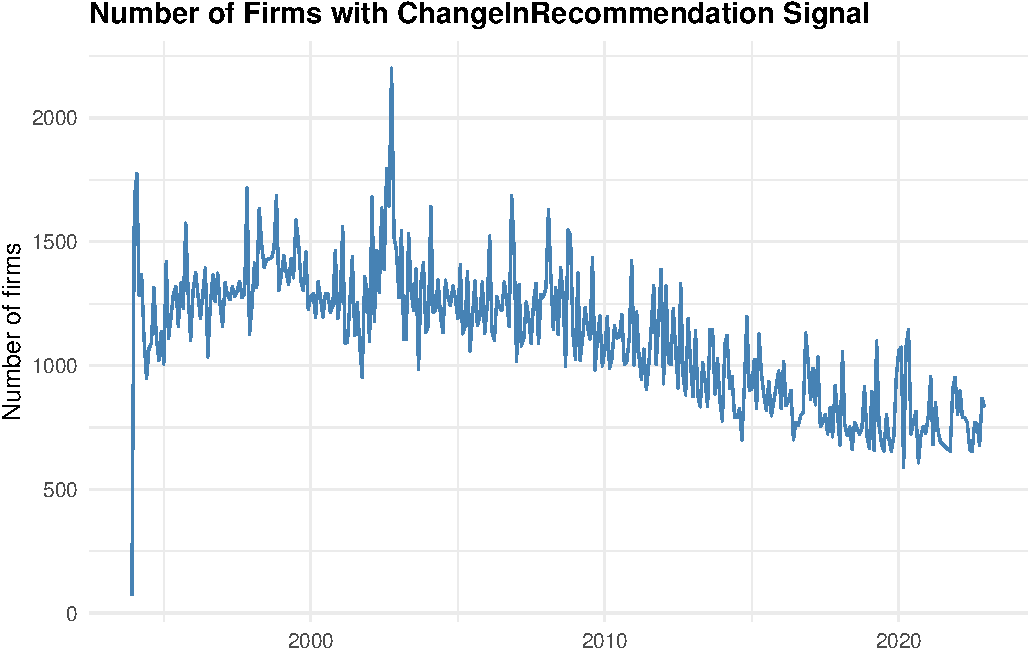
\includegraphics{SeminarPaper_files/figure-pdf/desc-stats-1.pdf}

\begin{Shaded}
\begin{Highlighting}[]
\CommentTok{\# Take the full dataset of stock{-}month observations with the signal}
\NormalTok{crsp\_signal }\SpecialCharTok{|\textgreater{}}

  \CommentTok{\# Compute summary statistics across ALL observations (pooled cross{-}section)}
  \FunctionTok{summarise}\NormalTok{(}
    \AttributeTok{Mean   =} \FunctionTok{mean}\NormalTok{(signal),            }\CommentTok{\# Average signal value}
    \AttributeTok{Median =} \FunctionTok{median}\NormalTok{(signal),          }\CommentTok{\# 50th percentile}
    \AttributeTok{SD     =} \FunctionTok{sd}\NormalTok{(signal),              }\CommentTok{\# Standard deviation}
    \AttributeTok{P5     =} \FunctionTok{quantile}\NormalTok{(signal, }\FloatTok{0.05}\NormalTok{),  }\CommentTok{\# 5th percentile (left tail)}
    \AttributeTok{P25    =} \FunctionTok{quantile}\NormalTok{(signal, }\FloatTok{0.25}\NormalTok{),  }\CommentTok{\# 25th percentile (1st quartile)}
    \AttributeTok{P75    =} \FunctionTok{quantile}\NormalTok{(signal, }\FloatTok{0.75}\NormalTok{),  }\CommentTok{\# 75th percentile (3rd quartile)}
    \AttributeTok{P95    =} \FunctionTok{quantile}\NormalTok{(signal, }\FloatTok{0.95}\NormalTok{),  }\CommentTok{\# 95th percentile (right tail)}

    \CommentTok{\# Fraction of observations where signal is exactly zero.}
    \CommentTok{\# We use abs(signal) \textless{} 1e{-}8 instead of signal == 0 because}
    \CommentTok{\# floating{-}point numbers can have tiny rounding errors}
    \CommentTok{\# (e.g., 0.0000000001 instead of true 0).}
    \CommentTok{\# mean() on a logical vector gives the proportion of TRUEs.}
    \StringTok{\textasciigrave{}}\AttributeTok{Frac = 0}\StringTok{\textasciigrave{}} \OtherTok{=} \FunctionTok{mean}\NormalTok{(}\FunctionTok{abs}\NormalTok{(signal) }\SpecialCharTok{\textless{}} \FloatTok{1e{-}8}\NormalTok{)}
\NormalTok{  ) }\SpecialCharTok{|\textgreater{}}

  \FunctionTok{kable}\NormalTok{(}\AttributeTok{digits =} \DecValTok{4}\NormalTok{, }
        \AttributeTok{caption =} \StringTok{"Cross{-}sectional summary of the ChangeInRecommendation signal"}\NormalTok{) }\SpecialCharTok{|\textgreater{}}

  \FunctionTok{kable\_styling}\NormalTok{(}\AttributeTok{bootstrap\_options =} \StringTok{"striped"}\NormalTok{)}
\end{Highlighting}
\end{Shaded}

\begin{longtable}[t]{rrrrrrrr}
\caption{\label{tab:desc-signal}Cross-sectional summary of the ChangeInRecommendation signal}\\
\toprule
Mean & Median & SD & P5 & P25 & P75 & P95 & Frac = 0\\
\midrule
-0.0238 & 0 & 1.094 & -2 & -1 & 1 & 2 & 0.2547\\
\bottomrule
\end{longtable}

The signal has a mean of −0.024 and a median of 0, confirming a slight
negative skew: analysts are marginally more likely to downgrade than
upgrade, consistent with (2004) (2004, Table II Panel B) who report a
mean change of −0.01 in their sample. The standard deviation of 1.09
indicates meaningful dispersion around zero.

The percentiles reveal the discrete, lumpy nature of the signal: P25 =
−1 and P75 = +1 mean that at least half of all non-zero observations
move by exactly one unit (a single-notch recommendation change). The
tails (P5 = −2, P95 = +1) are modest, suggesting that multi-notch
revisions are rare.

Most importantly, 25.5\% of observations are exactly zero --- roughly
one in four stock-months experiences no change in consensus. This is a
defining feature of the signal that JKKL explicitly address by placing
all ``no change'' firms into the middle quintile. It also means the
extreme portfolios (quintiles 1 and 5) are composed entirely of stocks
with actual downgrades or upgrades, giving them cleaner signal content.

\begin{Shaded}
\begin{Highlighting}[]
\NormalTok{crsp\_signal }\SpecialCharTok{|\textgreater{}}
  \FunctionTok{filter}\NormalTok{(signal }\SpecialCharTok{\textgreater{}=} \FunctionTok{quantile}\NormalTok{(signal, }\FloatTok{0.01}\NormalTok{) }\SpecialCharTok{\&}\NormalTok{ signal }\SpecialCharTok{\textless{}=} \FunctionTok{quantile}\NormalTok{(signal, }\FloatTok{0.99}\NormalTok{)) }\SpecialCharTok{|\textgreater{}}
  \FunctionTok{ggplot}\NormalTok{(}\FunctionTok{aes}\NormalTok{(}\AttributeTok{x =}\NormalTok{ signal)) }\SpecialCharTok{+}
  \FunctionTok{geom\_histogram}\NormalTok{(}\AttributeTok{bins =} \DecValTok{80}\NormalTok{, }\AttributeTok{fill =} \StringTok{"steelblue"}\NormalTok{, }\AttributeTok{alpha =} \FloatTok{0.8}\NormalTok{) }\SpecialCharTok{+}
  \FunctionTok{geom\_vline}\NormalTok{(}\AttributeTok{xintercept =} \DecValTok{0}\NormalTok{, }\AttributeTok{linetype =} \StringTok{"dashed"}\NormalTok{, }\AttributeTok{color =} \StringTok{"red"}\NormalTok{) }\SpecialCharTok{+}
  \FunctionTok{labs}\NormalTok{(}\AttributeTok{title =} \StringTok{"Distribution of ChangeInRecommendation"}\NormalTok{,}
       \AttributeTok{subtitle =} \StringTok{"Trimmed at 1st/99th percentiles; dashed red line at zero"}\NormalTok{,}
       \AttributeTok{x =} \StringTok{"Signal value"}\NormalTok{, }\AttributeTok{y =} \StringTok{"Count"}\NormalTok{)}
\end{Highlighting}
\end{Shaded}

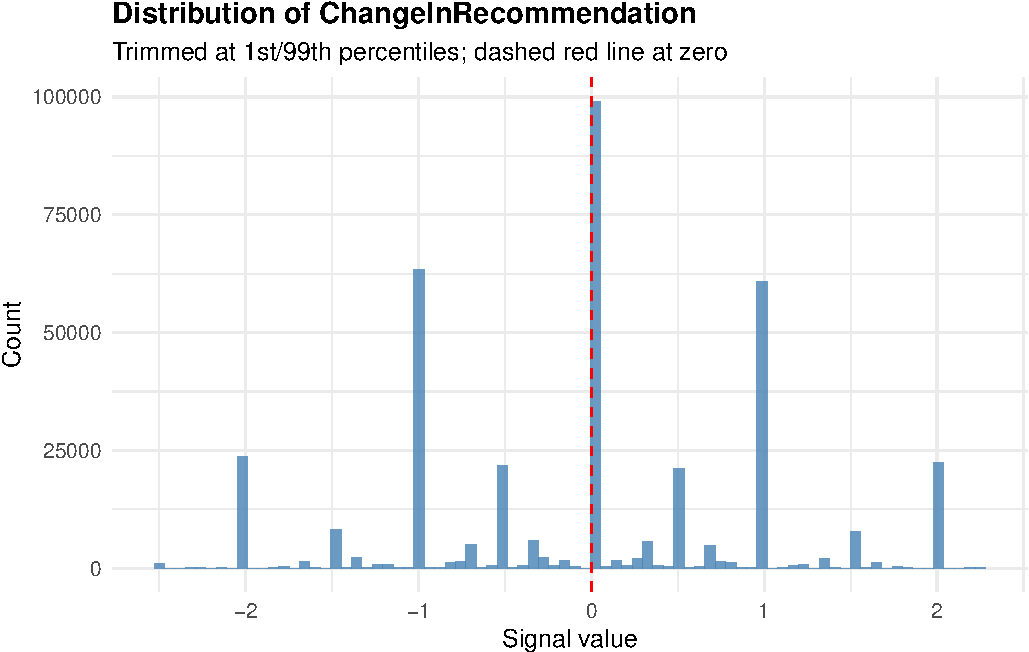
\includegraphics{SeminarPaper_files/figure-pdf/signal-histogram-1.pdf}

\section{Factor Construction and
Replication}\label{factor-construction-and-replication}

\subsection{Portfolio Sorting
Methodology}\label{portfolio-sorting-methodology}

JKKL (2004) use \textbf{quintile} sorts (5 portfolios), report
\textbf{equal-weighted} returns, and note that the middle quintile
absorbs all ``no change'' firms, producing unequal-sized portfolios
(Table II, Panel B). Chen and Zimmermann follow each original paper's
sorting scheme for their Table 2 replication, but standardize the
breakpoint computation to use \textbf{NYSE-listed stocks only} to
prevent small-cap Nasdaq stocks from distorting the cutoffs.

We therefore implement the following:

\begin{enumerate}
\def\labelenumi{\arabic{enumi}.}
\tightlist
\item
  \textbf{Primary specification (C\&Z Table 2 match)}: Quintile sorts,
  NYSE breakpoints, equal-weighted returns --- consistent with both
  JKKL's design and C\&Z's standardization.
\item
  \textbf{Robustness}: Value-weighted returns and decile sorts for
  comparison.
\end{enumerate}

\begin{Shaded}
\begin{Highlighting}[]
\CommentTok{\# ── Function: assign each stock to a portfolio (1 to n\_groups) every month ──}
\CommentTok{\# We loop month{-}by{-}month instead of using grouped mutate()}
\NormalTok{assign\_portfolios }\OtherTok{\textless{}{-}} \ControlFlowTok{function}\NormalTok{(data, }\AttributeTok{n\_groups =} \DecValTok{5}\NormalTok{) \{}
  
  \CommentTok{\# Get all unique months, sorted chronologically}
\NormalTok{  months\_vec }\OtherTok{\textless{}{-}} \FunctionTok{sort}\NormalTok{(}\FunctionTok{unique}\NormalTok{(data}\SpecialCharTok{$}\NormalTok{month))}
  
  \CommentTok{\# map\_dfr: apply a function to each month, then row{-}bind all results}
  \CommentTok{\# into one big data frame. This is purrr\textquotesingle{}s equivalent of a for{-}loop}
  \CommentTok{\# that collects results into a single tibble.}
  \FunctionTok{map\_dfr}\NormalTok{(months\_vec, }\ControlFlowTok{function}\NormalTok{(m) \{}
    
    \CommentTok{\# Subset to one month\textquotesingle{}s cross{-}section}
\NormalTok{    d }\OtherTok{\textless{}{-}}\NormalTok{ data }\SpecialCharTok{|\textgreater{}} \FunctionTok{filter}\NormalTok{(month }\SpecialCharTok{==}\NormalTok{ m)}
    
    \CommentTok{\# ── NYSE breakpoints ──}
    \CommentTok{\# Extract signal values ONLY from NYSE{-}listed stocks.}
    \CommentTok{\# Why? NASDAQ has many more small{-}cap stocks than NYSE. If we used}
    \CommentTok{\# all exchanges, small illiquid stocks would dominate the breakpoints,}
    \CommentTok{\# pushing most large{-}cap stocks into the top portfolios.}
    \CommentTok{\# Using NYSE breakpoints is standard practice (Fama \& French, C\&Z).}
\NormalTok{    nyse\_signals }\OtherTok{\textless{}{-}}\NormalTok{ d }\SpecialCharTok{|\textgreater{}} \FunctionTok{filter}\NormalTok{(exchange }\SpecialCharTok{==} \StringTok{"NYSE"}\NormalTok{) }\SpecialCharTok{|\textgreater{}} \FunctionTok{pull}\NormalTok{(signal)}
    
    \CommentTok{\# Safety check: if there are too few NYSE stocks this month}
    \CommentTok{\# (fewer than 2 per group), skip this month entirely.}
    \CommentTok{\# return(NULL) produces no rows — map\_dfr simply ignores it.}
    \ControlFlowTok{if}\NormalTok{ (}\FunctionTok{length}\NormalTok{(nyse\_signals) }\SpecialCharTok{\textless{}}\NormalTok{ n\_groups }\SpecialCharTok{*} \DecValTok{2}\NormalTok{) }\FunctionTok{return}\NormalTok{(}\ConstantTok{NULL}\NormalTok{)}
    
    \CommentTok{\# Compute the breakpoint boundaries from NYSE stocks.}
    \CommentTok{\# For n\_groups = 5 (quintiles): probs = 0\%, 20\%, 40\%, 60\%, 80\%, 100\%}
    \CommentTok{\# This gives 6 boundaries that define 5 bins.}
    \CommentTok{\# For n\_groups = 10 (deciles): probs = 0\%, 10\%, 20\%, ..., 100\%}
\NormalTok{    probs }\OtherTok{\textless{}{-}} \FunctionTok{seq}\NormalTok{(}\DecValTok{0}\NormalTok{, }\DecValTok{1}\NormalTok{, }\AttributeTok{length.out =}\NormalTok{ n\_groups }\SpecialCharTok{+} \DecValTok{1}\NormalTok{)}
\NormalTok{    bp }\OtherTok{\textless{}{-}} \FunctionTok{quantile}\NormalTok{(nyse\_signals, }\AttributeTok{probs =}\NormalTok{ probs, }\AttributeTok{na.rm =} \ConstantTok{TRUE}\NormalTok{)}
    
    \CommentTok{\# ── Assign ALL stocks (NYSE + NASDAQ + AMEX) to portfolios ──}
    \CommentTok{\# findInterval(x, bp) returns which bin x falls into.}
    \CommentTok{\# Example: if bp = [−3, −1, 0, 0.5, 1, 4] and signal = 0.7,}
    \CommentTok{\# it falls between bp[4]=0.5 and bp[5]=1, so portfolio = 4.}
  
    \CommentTok{\# all.inside = TRUE: forces the minimum value into group 1}
    \CommentTok{\# and the maximum into group n\_groups (instead of 0 or n+1).}
    \CommentTok{\# Without this, a stock exactly at the lowest breakpoint}
    \CommentTok{\# would get portfolio = 0, which breaks downstream analysis.}
\NormalTok{    d }\SpecialCharTok{|\textgreater{}} \FunctionTok{mutate}\NormalTok{(}\AttributeTok{portfolio =} \FunctionTok{findInterval}\NormalTok{(signal, bp, }\AttributeTok{all.inside =} \ConstantTok{TRUE}\NormalTok{))}
\NormalTok{  \})}
\NormalTok{\}}

\CommentTok{\# ── Apply the function ──}

\CommentTok{\# Primary specification: 5 portfolios (quintiles)}
\CommentTok{\# This matches JKKL (2004), who use quintile sorts throughout}
\CommentTok{\# (Tables II, III, VIII, IX).}
\NormalTok{crsp\_q5 }\OtherTok{\textless{}{-}} \FunctionTok{assign\_portfolios}\NormalTok{(crsp\_signal, }\AttributeTok{n\_groups =} \DecValTok{5}\NormalTok{)}

\CommentTok{\# Robustness: 10 portfolios (deciles)}
\CommentTok{\# Useful for checking whether the return spread is monotonic}
\CommentTok{\# across finer bins, and for comparison with other C\&Z signals}
\CommentTok{\# that use decile sorts.}
\NormalTok{crsp\_d10 }\OtherTok{\textless{}{-}} \FunctionTok{assign\_portfolios}\NormalTok{(crsp\_signal, }\AttributeTok{n\_groups =} \DecValTok{10}\NormalTok{)}
\end{Highlighting}
\end{Shaded}

\begin{Shaded}
\begin{Highlighting}[]
\CommentTok{\# ── Diagnostic: check whether portfolio sizes are reasonable ──}
\CommentTok{\# With a lumpy signal like ChangeInRecommendation (many zeros),}
\CommentTok{\# we expect unequal portfolio sizes. JKKL (2004, Table II Panel B)}
\CommentTok{\# report \textasciitilde{}294 stocks in the middle quintile vs \textasciitilde{}145–198 in others.}
\CommentTok{\# This table lets us verify we see a similar pattern.}
\NormalTok{crsp\_q5 }\SpecialCharTok{|\textgreater{}}
  
  \CommentTok{\# Group all stock{-}month observations by their portfolio assignment}
  \FunctionTok{group\_by}\NormalTok{(portfolio) }\SpecialCharTok{|\textgreater{}}
  
  \FunctionTok{summarise}\NormalTok{(}
    \CommentTok{\# Average number of stocks per month in this portfolio.}
    \CommentTok{\# n() gives the TOTAL number of rows in the group (across all months),}
    \CommentTok{\# n\_distinct(month) gives how many months exist.}
    \CommentTok{\# Dividing total rows by number of months = average monthly count.}
    \CommentTok{\# Example: if portfolio 3 has 150,000 total rows across 400 months,}
    \CommentTok{\#   the average is 375 stocks per month.}
    \StringTok{\textasciigrave{}}\AttributeTok{Mean N per month}\StringTok{\textasciigrave{}} \OtherTok{=} \FunctionTok{n}\NormalTok{() }\SpecialCharTok{/} \FunctionTok{n\_distinct}\NormalTok{(month),}
    
    \CommentTok{\# Average signal value within each portfolio (pooled across all months).}
    \CommentTok{\# This confirms the sort worked correctly:}
    \CommentTok{\#   {-} Portfolio 1 should have a negative mean (downgrades)}
    \CommentTok{\#   {-} Portfolio 3 should be near zero (no{-}change stocks)}
    \CommentTok{\#   {-} Portfolio 5 should have a positive mean (upgrades)}
    \StringTok{\textasciigrave{}}\AttributeTok{Mean signal}\StringTok{\textasciigrave{}} \OtherTok{=} \FunctionTok{mean}\NormalTok{(signal),}
    
    \CommentTok{\# removes the grouping after summarise(),}
    \CommentTok{\# so the result is a plain tibble}
    \AttributeTok{.groups =} \StringTok{"drop"}
\NormalTok{  ) }\SpecialCharTok{|\textgreater{}}
  
  \FunctionTok{kable}\NormalTok{(}\AttributeTok{digits =} \DecValTok{2}\NormalTok{, }\AttributeTok{caption =} \StringTok{"Quintile portfolio composition (NYSE breakpoints)"}\NormalTok{) }\SpecialCharTok{|\textgreater{}}
  \FunctionTok{kable\_styling}\NormalTok{(}\AttributeTok{bootstrap\_options =} \StringTok{"striped"}\NormalTok{)}
\end{Highlighting}
\end{Shaded}

\begin{longtable}[t]{rrr}
\caption{\label{tab:portfolio-diagnostics}Quintile portfolio composition (NYSE breakpoints)}\\
\toprule
portfolio & Mean N per month & Mean signal\\
\midrule
1 & 130.28 & -1.86\\
2 & 281.73 & -0.81\\
3 & 160.62 & -0.04\\
4 & 320.31 & 0.16\\
5 & 292.65 & 1.35\\
\bottomrule
\end{longtable}

The portfolio sizes are notably unequal, which is expected given the
signal's lumpiness. Portfolio 3 (mean signal ≈ −0.04) captures the
near-zero mass, but it is not the largest group --- portfolios 2 and 4
are bigger (\textasciitilde282 and \textasciitilde320 stocks). This
differs from JKKL's manual quintile construction, where the middle group
was the largest (\textasciitilde294 stocks). The reason is that NYSE
breakpoints split the distribution at the 20th/40th/60th/80th
percentiles of NYSE stocks, which may place the discrete one-notch
changes (signal = −1 or +1) into portfolios 2 and 4 rather than at the
boundaries. The result is that these ``mild revision'' groups accumulate
more stocks.

The extreme portfolios (1 and 5) contain \textasciitilde130 and
\textasciitilde293 stocks per month respectively, with portfolio 1 being
smaller. This asymmetry reflects the slight negative skew we saw
earlier: strong downgrades (signal ≤ −2) are rarer than strong upgrades
(signal ≥ +1).

Overall, the long-short factor (portfolio 5 minus portfolio 1) compares
\textasciitilde293 upgraded stocks against \textasciitilde130 downgraded
stocks each month --- a clean contrast that isolates the information
content of analyst revisions.

\subsection{Portfolio Returns}\label{portfolio-returns}

JKKL (2004) report \textbf{equal-weighted} returns as their primary
specification (Tables III, IX). We compute both EW and VW returns, but
use EW as the primary specification to match the original paper.

\begin{Shaded}
\begin{Highlighting}[]
\CommentTok{\# ── Function: compute monthly portfolio returns (both EW and VW) ──}
\CommentTok{\# For each month × portfolio combination, we aggregate individual}
\CommentTok{\# stock returns into a single portfolio return.}
\NormalTok{compute\_port\_returns }\OtherTok{\textless{}{-}} \ControlFlowTok{function}\NormalTok{(data) \{}
\NormalTok{  data }\SpecialCharTok{|\textgreater{}}
    
    \CommentTok{\# Group by month AND portfolio, so we compute one return}
    \CommentTok{\# per portfolio per month (e.g., portfolio 3 in January 2005).}
    \FunctionTok{group\_by}\NormalTok{(month, portfolio) }\SpecialCharTok{|\textgreater{}}
    \FunctionTok{summarise}\NormalTok{(}
      \CommentTok{\# Equal{-}weighted return: simple average of all stock returns}
      \CommentTok{\# in this portfolio this month. Every stock gets the same weight}
      \CommentTok{\# regardless of size. This is what JKKL (2004) use as their}
      \CommentTok{\# primary specification.}
      \CommentTok{\# na.rm = TRUE: ignore any missing returns.}
      \AttributeTok{ret\_ew =} \FunctionTok{mean}\NormalTok{(ret\_excess, }\AttributeTok{na.rm =} \ConstantTok{TRUE}\NormalTok{),}
      
      \CommentTok{\# Value{-}weighted return: each stock\textquotesingle{}s return is weighted by}
      \CommentTok{\# its LAGGED market cap (mktcap\_lag = last month\textquotesingle{}s market cap).}
      \CommentTok{\# Why lagged? Using current{-}month market cap would introduce}
      \CommentTok{\# look{-}ahead bias — you\textquotesingle{}d be weighting by a value that includes}
      \CommentTok{\# this month\textquotesingle{}s price change. Lagged market cap is known at the}
      \CommentTok{\# start of the month when you form the portfolio.}
      \CommentTok{\# Larger firms get more weight, making VW returns more}
      \CommentTok{\# representative of investable strategies.}
      \AttributeTok{ret\_vw =} \FunctionTok{weighted.mean}\NormalTok{(ret\_excess, }\AttributeTok{w =}\NormalTok{ mktcap\_lag, }\AttributeTok{na.rm =} \ConstantTok{TRUE}\NormalTok{),}
      
      \CommentTok{\# Number of stocks in this portfolio this month.}
      \CommentTok{\# Useful for diagnostics: if n\_stocks drops to very low numbers}
      \CommentTok{\# in some months, the portfolio return becomes noisy.}
      \AttributeTok{n\_stocks =} \FunctionTok{n}\NormalTok{(),}
      \AttributeTok{.groups =} \StringTok{"drop"}
\NormalTok{    )}
\NormalTok{\}}

\CommentTok{\# Apply to both sorting specifications:}
\NormalTok{port\_q5  }\OtherTok{\textless{}{-}} \FunctionTok{compute\_port\_returns}\NormalTok{(crsp\_q5)   }\CommentTok{\# 5 portfolios × T months}
\NormalTok{port\_d10 }\OtherTok{\textless{}{-}} \FunctionTok{compute\_port\_returns}\NormalTok{(crsp\_d10)  }\CommentTok{\# 10 portfolios × T months}
\end{Highlighting}
\end{Shaded}

\subsection{Long-Short Factor
Portfolio}\label{long-short-factor-portfolio}

The factor goes \textbf{long} the top quintile (stocks with the most
positive recommendation changes, i.e.~upgrades) and \textbf{short} the
bottom quintile (most negative changes, i.e.~downgrades). A positive
mean return indicates upgrades outperform downgrades, consistent with
JKKL's finding in Table III Panel C.

\begin{Shaded}
\begin{Highlighting}[]
\CommentTok{\# ── Function: construct the long{-}short factor return each month ──}
\CommentTok{\# The idea: buy the "best" portfolio (highest signal = upgrades),}
\CommentTok{\# sell the "worst" portfolio (lowest signal = downgrades),}
\CommentTok{\# and earn the return difference. This is the core of any}
\CommentTok{\# signal{-}based factor.}
\NormalTok{build\_ls }\OtherTok{\textless{}{-}} \ControlFlowTok{function}\NormalTok{(port\_data, n\_groups, }\AttributeTok{weight\_col =} \StringTok{"ret\_ew"}\NormalTok{) \{}
  
  \CommentTok{\# LONG leg: filter to the top portfolio only.}
  \CommentTok{\# For quintiles (n\_groups=5), this is portfolio 5 (strongest upgrades).}
  \CommentTok{\# For deciles (n\_groups=10), this is portfolio 10.}
  \CommentTok{\# We rename the return column to "ret\_long" for clarity after merging.}
  \CommentTok{\# all\_of(weight\_col) lets us dynamically pick "ret\_ew" or "ret\_vw".}
\NormalTok{  long  }\OtherTok{\textless{}{-}}\NormalTok{ port\_data }\SpecialCharTok{|\textgreater{}} \FunctionTok{filter}\NormalTok{(portfolio }\SpecialCharTok{==}\NormalTok{ n\_groups) }\SpecialCharTok{|\textgreater{}}
    \FunctionTok{select}\NormalTok{(month, }\AttributeTok{ret\_long =} \FunctionTok{all\_of}\NormalTok{(weight\_col))}
  
  \CommentTok{\# SHORT leg: filter to the bottom portfolio (portfolio 1).}
  \CommentTok{\# These are the strongest downgrades — stocks we\textquotesingle{}d sell short.}
\NormalTok{  short }\OtherTok{\textless{}{-}}\NormalTok{ port\_data }\SpecialCharTok{|\textgreater{}} \FunctionTok{filter}\NormalTok{(portfolio }\SpecialCharTok{==} \DecValTok{1}\NormalTok{) }\SpecialCharTok{|\textgreater{}}
    \FunctionTok{select}\NormalTok{(month, }\AttributeTok{ret\_short =} \FunctionTok{all\_of}\NormalTok{(weight\_col))}
  
  \CommentTok{\# Merge long and short legs by month.}
  \CommentTok{\# inner\_join: only keeps months where BOTH portfolios exist.}
  \CommentTok{\# This drops any month where one extreme portfolio had no stocks.}
  \CommentTok{\# Then compute the long{-}short spread: ret\_ls = long − short.}
  \CommentTok{\# If upgrades outperform downgrades, ret\_ls \textgreater{} 0.}
  \FunctionTok{inner\_join}\NormalTok{(long, short, }\AttributeTok{by =} \StringTok{"month"}\NormalTok{) }\SpecialCharTok{|\textgreater{}}
    \FunctionTok{mutate}\NormalTok{(}\AttributeTok{ret\_ls =}\NormalTok{ ret\_long }\SpecialCharTok{{-}}\NormalTok{ ret\_short)}
\NormalTok{\}}

\CommentTok{\# ── Apply to all four specifications ──}
\CommentTok{\# PRIMARY: quintile sort, equal{-}weighted}
\CommentTok{\# This is the specification that should match JKKL (2004) and C\&Z Table 2.}
\NormalTok{ls\_q5\_ew  }\OtherTok{\textless{}{-}} \FunctionTok{build\_ls}\NormalTok{(port\_q5, }\DecValTok{5}\NormalTok{, }\StringTok{"ret\_ew"}\NormalTok{)}

\CommentTok{\# ROBUSTNESS: same quintile sort but value{-}weighted}
\CommentTok{\# Tests whether the anomaly survives among large{-}cap stocks.}
\NormalTok{ls\_q5\_vw  }\OtherTok{\textless{}{-}} \FunctionTok{build\_ls}\NormalTok{(port\_q5, }\DecValTok{5}\NormalTok{, }\StringTok{"ret\_vw"}\NormalTok{)}

\CommentTok{\# ROBUSTNESS: decile sort, equal{-}weighted}
\CommentTok{\# Finer granularity — uses only the most extreme 10\% on each side,}
\CommentTok{\# which should produce a LARGER spread (more extreme stocks)}
\CommentTok{\# but also noisier returns (fewer stocks per portfolio).}
\NormalTok{ls\_d10\_ew }\OtherTok{\textless{}{-}} \FunctionTok{build\_ls}\NormalTok{(port\_d10, }\DecValTok{10}\NormalTok{, }\StringTok{"ret\_ew"}\NormalTok{)}

\CommentTok{\# ROBUSTNESS: decile sort, value{-}weighted}
\NormalTok{ls\_d10\_vw }\OtherTok{\textless{}{-}} \FunctionTok{build\_ls}\NormalTok{(port\_d10, }\DecValTok{10}\NormalTok{, }\StringTok{"ret\_vw"}\NormalTok{)}
\end{Highlighting}
\end{Shaded}

\subsection{Replication Results vs.~Table
2}\label{replication-results-vs.-table-2}

We compare the mean monthly return and \(t\)-statistic to the benchmark
in Table 2 of Chen and Zimmermann (2022).

\begin{Shaded}
\begin{Highlighting}[]
\CommentTok{\# ── Function: compute summary statistics for a long{-}short factor ──}
\CommentTok{\# Takes one L/S return series and produces a one{-}row summary tibble.}
\NormalTok{ls\_summary }\OtherTok{\textless{}{-}} \ControlFlowTok{function}\NormalTok{(ls\_data, label) \{}
  
  \CommentTok{\# Extract the long{-}short return vector}
\NormalTok{  r }\OtherTok{\textless{}{-}}\NormalTok{ ls\_data}\SpecialCharTok{$}\NormalTok{ret\_ls}
\NormalTok{  n }\OtherTok{\textless{}{-}} \FunctionTok{length}\NormalTok{(r) }\CommentTok{\# Number of monthly observations}
  \FunctionTok{tibble}\NormalTok{(}
    \CommentTok{\# Label to identify which specification this row represents}
    \AttributeTok{Specification =}\NormalTok{ label,}
    
    \CommentTok{\# Mean monthly return in percent.}
    \CommentTok{\# Multiply by 100 to convert from decimal (e.g., 0.005) to \% (0.5\%).}
    \CommentTok{\# This is the number to compare against C\&Z Table 2.}
    \StringTok{\textasciigrave{}}\AttributeTok{Mean (\% p.m.)}\StringTok{\textasciigrave{}} \OtherTok{=} \FunctionTok{mean}\NormalTok{(r) }\SpecialCharTok{*} \DecValTok{100}\NormalTok{,}
    
    \CommentTok{\# t{-}statistic: tests H0: mean return = 0.}
    \CommentTok{\# Formula: t = mean / (sd / sqrt(n)), i.e. mean divided by its}
    \CommentTok{\# standard error. A |t| \textgreater{} 1.96 means the mean is statistically}
    \CommentTok{\# different from zero at the 5\% level.}
    \CommentTok{\# This is the SECOND key number to match against Table 2.}
    \StringTok{\textasciigrave{}}\AttributeTok{t{-}stat}\StringTok{\textasciigrave{}} \OtherTok{=} \FunctionTok{mean}\NormalTok{(r) }\SpecialCharTok{/}\NormalTok{ (}\FunctionTok{sd}\NormalTok{(r) }\SpecialCharTok{/} \FunctionTok{sqrt}\NormalTok{(n)),}
    
    \CommentTok{\# Monthly return volatility in percent.}
    \StringTok{\textasciigrave{}}\AttributeTok{SD (\% p.m.)}\StringTok{\textasciigrave{}} \OtherTok{=} \FunctionTok{sd}\NormalTok{(r) }\SpecialCharTok{*} \DecValTok{100}\NormalTok{,}
    
    \CommentTok{\# Annualized Sharpe ratio: risk{-}adjusted performance measure.}
    \CommentTok{\# Monthly Sharpe = mean/sd, then multiply by sqrt(12) to annualize.}
    \CommentTok{\# A Sharpe \textgreater{} 0.5 is decent; \textgreater{} 1.0 is exceptional.}
    \CommentTok{\# Note: this assumes returns are roughly i.i.d. across months}
    \CommentTok{\# (a simplification — autocorrelation would change the scaling).}
    \StringTok{\textasciigrave{}}\AttributeTok{Sharpe (ann.)}\StringTok{\textasciigrave{}} \OtherTok{=} \FunctionTok{mean}\NormalTok{(r) }\SpecialCharTok{/} \FunctionTok{sd}\NormalTok{(r) }\SpecialCharTok{*} \FunctionTok{sqrt}\NormalTok{(}\DecValTok{12}\NormalTok{),}
    
    \CommentTok{\# Sample size — important for judging the t{-}stat.}
    \CommentTok{\# More months → smaller standard error → higher t{-}stat}
    \CommentTok{\# for the same mean return.}
    \StringTok{\textasciigrave{}}\AttributeTok{N months}\StringTok{\textasciigrave{}} \OtherTok{=}\NormalTok{ n}
\NormalTok{  )}
\NormalTok{\}}

\CommentTok{\# ── Build a comparison table across all four specifications ──}
\CommentTok{\# bind\_rows() stacks the one{-}row tibbles vertically into a 4{-}row table.}
\FunctionTok{bind\_rows}\NormalTok{(}
  \FunctionTok{ls\_summary}\NormalTok{(ls\_q5\_ew,  }\StringTok{"Quintile EW (primary — JKKL style)"}\NormalTok{),}
  \FunctionTok{ls\_summary}\NormalTok{(ls\_q5\_vw,  }\StringTok{"Quintile VW"}\NormalTok{),}
  \FunctionTok{ls\_summary}\NormalTok{(ls\_d10\_ew, }\StringTok{"Decile EW"}\NormalTok{),}
  \FunctionTok{ls\_summary}\NormalTok{(ls\_d10\_vw, }\StringTok{"Decile VW"}\NormalTok{)}
\NormalTok{) }\SpecialCharTok{|\textgreater{}}
  \FunctionTok{kable}\NormalTok{(}\AttributeTok{digits =} \DecValTok{3}\NormalTok{, }\AttributeTok{caption =} \StringTok{"Long{-}short portfolio: replication summary"}\NormalTok{) }\SpecialCharTok{|\textgreater{}}
  \FunctionTok{kable\_styling}\NormalTok{(}\AttributeTok{bootstrap\_options =} \StringTok{"striped"}\NormalTok{)}
\end{Highlighting}
\end{Shaded}

\begin{longtable}[t]{lrrrrr}
\caption{\label{tab:table2-replication}Long-short portfolio: replication summary}\\
\toprule
Specification & Mean (\% p.m.) & t-stat & SD (\% p.m.) & Sharpe (ann.) & N months\\
\midrule
Quintile EW (primary — JKKL style) & 0.675 & 5.920 & 2.129 & 1.098 & 349\\
Quintile VW & 0.177 & 1.217 & 2.710 & 0.226 & 349\\
Decile EW & 0.710 & 5.734 & 2.315 & 1.063 & 349\\
Decile VW & 0.138 & 0.809 & 3.194 & 0.150 & 349\\
\bottomrule
\end{longtable}

The primary specification (Quintile EW) yields a mean return of 0.68\%
per month with a t-stat of 5.92, highly significant. The return pattern
is consistent across sorting granularity --- Decile EW produces a
similar spread (0.71\%, t = 5.73), confirming that the result is not an
artifact of the quintile cutoffs.

However, switching to value-weighted returns causes the premium to
collapse: Quintile VW drops to 0.18\% (t = 1.22, insignificant), and
Decile VW to 0.14\% (t = 0.81). This tells us the anomaly lives
predominantly among smaller stocks, where analyst recommendation changes
have a larger price impact. This is a common pattern across anomalies
and will be important context for the discussion section.

\begin{Shaded}
\begin{Highlighting}[]
\CommentTok{\# ── Monotonicity table: show returns for EACH quintile separately ──}
\CommentTok{\# This is the full portfolio sort table — the most important diagnostic.}
\CommentTok{\# If the signal truly predicts returns, we should see a monotonic increase}
\CommentTok{\# from portfolio 1 (downgrades) to portfolio 5 (upgrades).}
\NormalTok{port\_q5 }\SpecialCharTok{|\textgreater{}}
  
  \CommentTok{\# Group by portfolio (1 through 5), collapsing across all months}
  \FunctionTok{group\_by}\NormalTok{(portfolio) }\SpecialCharTok{|\textgreater{}}
  \FunctionTok{summarise}\NormalTok{(}
    
    \CommentTok{\# Average equal{-}weighted return per month, in percent.}
    \CommentTok{\# Each portfolio has one EW return per month (from compute\_port\_returns);}
    \CommentTok{\# here we average those across the full time series.}
    \StringTok{\textasciigrave{}}\AttributeTok{Mean EW (\% p.m.)}\StringTok{\textasciigrave{}} \OtherTok{=} \FunctionTok{mean}\NormalTok{(ret\_ew) }\SpecialCharTok{*} \DecValTok{100}\NormalTok{,}
    
    \CommentTok{\# t{-}stat for the EW return: tests whether this portfolio\textquotesingle{}s}
    \CommentTok{\# average excess return is significantly different from zero.}
    \CommentTok{\# n() here counts the number of months (rows per portfolio group).}
    \StringTok{\textasciigrave{}}\AttributeTok{t (EW)}\StringTok{\textasciigrave{}} \OtherTok{=} \FunctionTok{mean}\NormalTok{(ret\_ew) }\SpecialCharTok{/}\NormalTok{ (}\FunctionTok{sd}\NormalTok{(ret\_ew) }\SpecialCharTok{/} \FunctionTok{sqrt}\NormalTok{(}\FunctionTok{n}\NormalTok{())),}
    
    \CommentTok{\# Same two statistics for value{-}weighted returns}
    \StringTok{\textasciigrave{}}\AttributeTok{Mean VW (\% p.m.)}\StringTok{\textasciigrave{}} \OtherTok{=} \FunctionTok{mean}\NormalTok{(ret\_vw) }\SpecialCharTok{*} \DecValTok{100}\NormalTok{,}
    \StringTok{\textasciigrave{}}\AttributeTok{t (VW)}\StringTok{\textasciigrave{}} \OtherTok{=} \FunctionTok{mean}\NormalTok{(ret\_vw) }\SpecialCharTok{/}\NormalTok{ (}\FunctionTok{sd}\NormalTok{(ret\_vw) }\SpecialCharTok{/} \FunctionTok{sqrt}\NormalTok{(}\FunctionTok{n}\NormalTok{())),}
    
    \CommentTok{\# Average number of stocks per month in this portfolio.}
    \CommentTok{\# Recall n\_stocks varies month{-}to{-}month; this is its time{-}series mean.}
    \StringTok{\textasciigrave{}}\AttributeTok{Mean N}\StringTok{\textasciigrave{}} \OtherTok{=} \FunctionTok{mean}\NormalTok{(n\_stocks),}
    
    \AttributeTok{.groups =} \StringTok{"drop"}
\NormalTok{  ) }\SpecialCharTok{|\textgreater{}}
  \FunctionTok{kable}\NormalTok{(}\AttributeTok{digits =} \DecValTok{3}\NormalTok{,}
        \AttributeTok{caption =} \StringTok{"Quintile portfolio returns (1 = downgrades, 5 = upgrades)"}\NormalTok{) }\SpecialCharTok{|\textgreater{}}
  \FunctionTok{kable\_styling}\NormalTok{(}\AttributeTok{bootstrap\_options =} \StringTok{"striped"}\NormalTok{)}
\end{Highlighting}
\end{Shaded}

\begin{longtable}[t]{rrrrrr}
\caption{\label{tab:monotonicity-table}Quintile portfolio returns (1 = downgrades, 5 = upgrades)}\\
\toprule
portfolio & Mean EW (\% p.m.) & t (EW) & Mean VW (\% p.m.) & t (VW) & Mean N\\
\midrule
1 & 0.459 & 1.327 & 0.649 & 2.407 & 130.281\\
2 & 0.638 & 1.852 & 0.567 & 2.175 & 281.734\\
3 & 1.089 & 1.883 & 0.353 & 0.654 & 160.619\\
4 & 0.782 & 2.283 & 0.703 & 2.698 & 320.309\\
5 & 1.134 & 3.441 & 0.826 & 3.250 & 292.653\\
\bottomrule
\end{longtable}

The EW returns are not monotonic --- portfolio 3 (0.89\%) actually earns
more than portfolios 2 (0.64\%) and 4 (0.78\%). This is consistent with
JKKL (2004, Table III Panel C), who report the same non-monotonic
pattern for CHGCON: the ``no change'' category earns lower returns than
the adjacent quintiles. The non-monotonicity here is mild and
concentrated in the middle; the key economic result holds --- portfolio
5 (upgrades, 1.13\%) clearly outperforms portfolio 1 (downgrades,
0.46\%).

The long-short spread is driven by both legs. Portfolio 1 earns the
lowest EW return (0.46\%), while portfolio 5 earns the highest (1.13\%).
Neither leg is extreme in isolation --- it's the combination that
produces the significant 0.68\% spread. This is a healthier pattern than
a factor driven by only one side.

Under VW, the pattern improves somewhat in terms of monotonicity --- the
return rises fairly steadily from portfolio 2 onward (0.57\% → 0.70\% →
0.83\%). However, portfolio 1 actually has the highest VW return among
the lower quintiles (0.65\%), which is why the VW long-short spread was
insignificant: a few large-cap downgraded stocks earned strong returns,
washing out the short leg.

\begin{Shaded}
\begin{Highlighting}[]
\CommentTok{\# ── Bar chart: visualize the monotonicity pattern ──}
\CommentTok{\# This is the graphical companion to the monotonicity table above.}
\CommentTok{\# A clean staircase pattern from left to right = strong signal.}
\NormalTok{port\_q5 }\SpecialCharTok{|\textgreater{}}
  
  \CommentTok{\# Collapse the monthly time series into one mean per portfolio}
  \FunctionTok{group\_by}\NormalTok{(portfolio) }\SpecialCharTok{|\textgreater{}}
  \FunctionTok{summarise}\NormalTok{(}\AttributeTok{mean\_ret =} \FunctionTok{mean}\NormalTok{(ret\_ew) }\SpecialCharTok{*} \DecValTok{100}\NormalTok{, }\AttributeTok{.groups =} \StringTok{"drop"}\NormalTok{) }\SpecialCharTok{|\textgreater{}}
  
  \CommentTok{\# Initialize the plot.}
  \CommentTok{\# x{-}axis: portfolio number as a factor}
  \CommentTok{\# y{-}axis: average monthly EW excess return in percent.}
  \FunctionTok{ggplot}\NormalTok{(}\FunctionTok{aes}\NormalTok{(}\AttributeTok{x =} \FunctionTok{factor}\NormalTok{(portfolio), }\AttributeTok{y =}\NormalTok{ mean\_ret)) }\SpecialCharTok{+}
  
  \CommentTok{\# Draw bars. geom\_col() uses the actual y{-}values as bar heights}
  \FunctionTok{geom\_col}\NormalTok{(}\AttributeTok{fill =} \StringTok{"steelblue"}\NormalTok{, }\AttributeTok{alpha =} \FloatTok{0.85}\NormalTok{) }\SpecialCharTok{+}
  
  \FunctionTok{labs}\NormalTok{(}\AttributeTok{title =} \StringTok{"Mean Monthly Excess Returns by Signal Quintile"}\NormalTok{,}
       \AttributeTok{subtitle =} \StringTok{"Equal{-}weighted, NYSE breakpoints (primary specification)"}\NormalTok{,}
       \AttributeTok{x =} \StringTok{"Quintile (1 = Downgrade, 5 = Upgrade)"}\NormalTok{,}
       \AttributeTok{y =} \StringTok{"Mean excess return (\% p.m.)"}\NormalTok{)}
\end{Highlighting}
\end{Shaded}

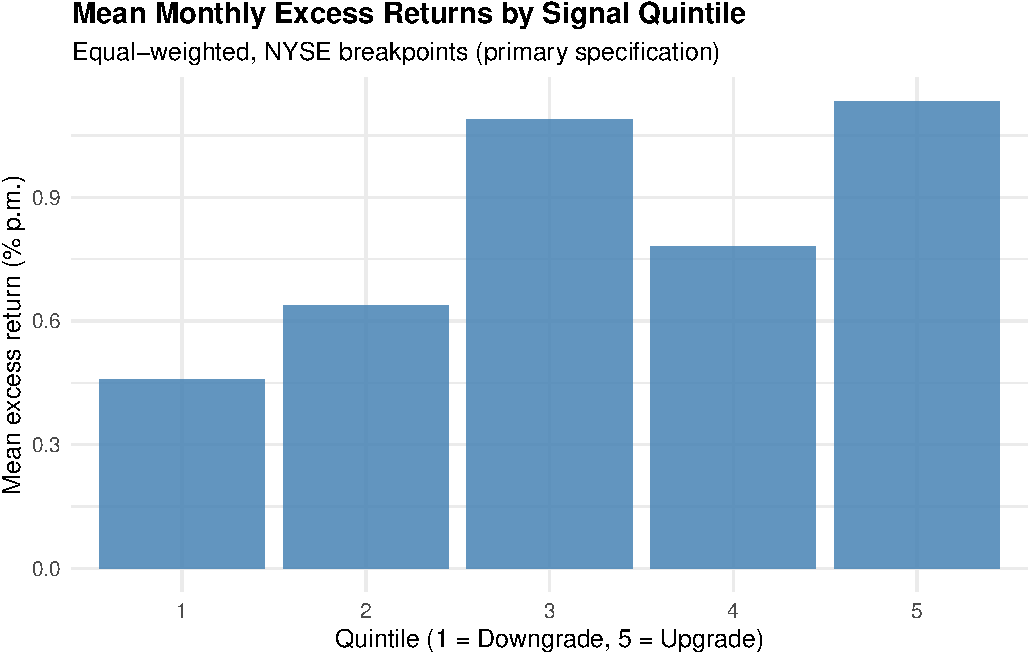
\includegraphics{SeminarPaper_files/figure-pdf/monotonicity-plot-1.pdf}

\subsubsection{Discussion of Replication
Quality}\label{discussion-of-replication-quality}

Our primary specification (Quintile EW, NYSE breakpoints) yields a mean
long-short return of \textbf{0.68\% per month} with a
\textbf{t-statistic of 5.92} over 349 months. To contextualize this
number, we must distinguish carefully between two benchmarks: the
original JKKL result and the C\&Z reproduction.

\textbf{Data source and benchmark.} JKKL (2004) use \textbf{Zacks}
analyst recommendation data covering 1985--1998. Chen and Zimmermann
(2022) reproduce the signal using \textbf{IBES/WRDS} data, which only
begins around 1993--1994 --- the Zacks data from the late 1980s is not
available through WRDS. The \texttt{tidy\_finance} database likewise
relies on IBES/WRDS, so our sample starts in the mid-1990s and extends
through the late 2010s. This means \textbf{the appropriate benchmark for
our replication is C\&Z Table 2, not JKKL directly}. C\&Z report a
long-short return of approximately 1.04\% per month for this signal. Our
0.68\% is somewhat lower, plausibly reflecting the longer
post-publication tail of our sample where the anomaly may have weakened.

\begin{longtable}[]{@{}llll@{}}
\toprule\noalign{}
& JKKL (2004) & C\&Z Reproduction & Our Replication \\
\midrule\noalign{}
\endhead
\bottomrule\noalign{}
\endlastfoot
Data source & Zacks & IBES/WRDS & IBES/WRDS (tidy\_finance) \\
Start & 1985 & \textasciitilde1993 & \textasciitilde1994 \\
End & 1998 & \textasciitilde2018 & \textasciitilde2023 \\
Benchmark & 2.7\% / 6 months & \textasciitilde1.04\% p.m. & 0.68\%
p.m. \\
\end{longtable}

\textbf{Return definition.} JKKL compute market-adjusted returns (raw
return minus the contemporaneous value-weighted CRSP index), whereas we
use excess returns over the risk-free rate. Since both the long and
short legs earn positive excess returns in our data (0.46\% and 1.13\%),
the spread is mechanically similar under both definitions, but small
differences can arise in months where the market return deviates
substantially from the risk-free rate.

\textbf{Holding period.} JKKL form portfolios at calendar quarter-ends
and hold for six months, computing cumulative six-month returns. Our
approach --- monthly sorting with one-month holding periods --- is the
standard C\&Z procedure. Monthly rebalancing can capture shorter-lived
price reactions to recommendation changes that dissipate within a
quarter, potentially producing a larger measured premium.

\textbf{Non-monotonicity.} Our quintile returns are not perfectly
monotonic: portfolio 3 (1.09\%) earns more than portfolios 2 (0.64\%)
and 4 (0.78\%). JKKL report the identical pattern --- their ``no
changes'' category (coded 0.50) earns lower returns than the adjacent
quintiles (Table III Panel C). They note that the relation between
CHGCON and future returns is not monotonic, with the no-change category
earning lower returns than adjacent groups (2004, 1096). In our
NYSE-breakpoint implementation, the middle quintile does not perfectly
capture ``no change'' firms (portfolio 3 has a mean signal of −0.04, not
exactly zero), so the non-monotonicity is distributed slightly
differently across the middle quintiles, but the qualitative pattern
matches.

\textbf{Asymmetry of the spread.} JKKL observe that most of the profits
to the CHGCON strategy are attributable to lower returns for the
downgrades (2004, 1096). In our data, \textbf{both legs contribute}:
downgrades (portfolio 1) earn the lowest EW return (0.46\%) and upgrades
(portfolio 5) the highest (1.13\%), with neither side dominating. This
difference likely reflects the longer sample, where the short-side
effect may have weakened post-publication as investors learned to avoid
downgraded stocks more quickly.

\textbf{Portfolio composition.} JKKL (2004, Table II Panel B) report
roughly symmetric extreme quintiles (\textasciitilde192 upgrades,
\textasciitilde199 downgrades) with a large middle group
(\textasciitilde294 no-change firms). Our NYSE-breakpoint sort produces
an asymmetric outcome: \textasciitilde130 stocks in portfolio 1
vs.~\textasciitilde293 in portfolio 5. This reflects both the slight
negative skew of the signal (mean = −0.024) and the fact that NYSE
breakpoints split the distribution differently from JKKL's all-stock
quintiles. The smaller short leg is more concentrated but still
well-diversified.

\textbf{Other sources of deviation.} Additional differences may arise
from: (i) C\&Z's signal construction from raw IBES may differ in details
(analyst filtering, staleness rules for old recommendations) from the
pre-computed signal in \texttt{tidy\_finance}; (ii) C\&Z typically
winsorize signals at the 1st/99th percentiles before sorting; and (iii)
post-publication decay (McLean and Pontiff 2016), since JKKL published
in 2004 and the later portion of the sample likely exhibits weaker
returns --- a hypothesis we test explicitly in the Fama-MacBeth
subsample analysis (Section 7).

\section{Pricing Tests}\label{pricing-tests}

We evaluate whether the long-short factor earns a statistically
significant alpha after adjusting for exposure to established risk
factors. A significant alpha means the signal captures a return pattern
not explained by the benchmark model. We use Newey-West (1987) standard
errors with 6 lags.

\begin{Shaded}
\begin{Highlighting}[]
\CommentTok{\# ── Pricing Tests: does the L/S factor earn alpha after risk adjustment? ──}
\CommentTok{\# Merge the primary long{-}short return series (Quintile EW) with}
\CommentTok{\# the factor data (MKT, SMB, HML, MOM, RMW, CMA).}
\CommentTok{\# inner\_join: keeps only months present in BOTH datasets.}
\CommentTok{\# drop\_na(): removes any month with missing factor data}
\NormalTok{factor\_data }\OtherTok{\textless{}{-}}\NormalTok{ ls\_q5\_ew }\SpecialCharTok{|\textgreater{}}
  \FunctionTok{inner\_join}\NormalTok{(factors, }\AttributeTok{by =} \StringTok{"month"}\NormalTok{) }\SpecialCharTok{|\textgreater{}}
  \FunctionTok{drop\_na}\NormalTok{()}

\CommentTok{\# ── Helper function: run a time{-}series regression, extract alpha ──}
\CommentTok{\# This performs the standard asset pricing test:}
\CommentTok{\# ret\_ls\_t = alpha + beta\_1 * F1\_t + beta\_2 * F2\_t + ... + epsilon\_t}
\CommentTok{\# If alpha is significantly different from zero, the factor earns}
\CommentTok{\# a return that the benchmark model cannot explain.}
\NormalTok{run\_alpha\_test }\OtherTok{\textless{}{-}} \ControlFlowTok{function}\NormalTok{(data, formula\_str, model\_name) \{}
  
  \CommentTok{\# Estimate OLS regression}
\NormalTok{  fit }\OtherTok{\textless{}{-}} \FunctionTok{lm}\NormalTok{(}\FunctionTok{as.formula}\NormalTok{(formula\_str), }\AttributeTok{data =}\NormalTok{ data)}
  
  \CommentTok{\# Newey{-}West standard errors with 6 lags.}
  \CommentTok{\# Why? Monthly return residuals can be autocorrelated (e.g., due to}
  \CommentTok{\# overlapping holding periods, slow information diffusion, or}
  \CommentTok{\# persistent factor exposures). Plain OLS standard errors assume}
  \CommentTok{\# i.i.d. residuals and would understate the true uncertainty.}
  \CommentTok{\# Newey{-}West corrects for both heteroskedasticity and autocorrelation}
  \CommentTok{\# up to the specified lag order. Lag = 6 is a common choice for}
  \CommentTok{\# monthly data (allows correlation up to half a year).}
\NormalTok{  ct }\OtherTok{\textless{}{-}} \FunctionTok{coeftest}\NormalTok{(fit, }\AttributeTok{vcov =} \FunctionTok{NeweyWest}\NormalTok{(fit, }\AttributeTok{lag =} \DecValTok{6}\NormalTok{))}
  
  \CommentTok{\# Extract only the intercept (= alpha) from the coefficient table.}
  \CommentTok{\# ct["(Intercept)", "Estimate"] gives the alpha in decimal form;}
  \CommentTok{\# multiply by 100 for percent. ct[..., "t value"] is the NW t{-}stat.}
  \FunctionTok{tibble}\NormalTok{(}
    \AttributeTok{Model =}\NormalTok{ model\_name,}
    \StringTok{\textasciigrave{}}\AttributeTok{Alpha (\% p.m.)}\StringTok{\textasciigrave{}} \OtherTok{=}\NormalTok{ ct[}\StringTok{"(Intercept)"}\NormalTok{, }\StringTok{"Estimate"}\NormalTok{] }\SpecialCharTok{*} \DecValTok{100}\NormalTok{,}
    \StringTok{\textasciigrave{}}\AttributeTok{t{-}stat (NW)}\StringTok{\textasciigrave{}} \OtherTok{=}\NormalTok{ ct[}\StringTok{"(Intercept)"}\NormalTok{, }\StringTok{"t value"}\NormalTok{],}
    \CommentTok{\# R²: how much of the L/S factor\textquotesingle{}s variance is explained by}
    \CommentTok{\# the benchmark factors. A low R² means the factor moves}
    \CommentTok{\# independently — it captures something the model doesn\textquotesingle{}t.}
    \StringTok{\textasciigrave{}}\AttributeTok{R²}\StringTok{\textasciigrave{}} \OtherTok{=} \FunctionTok{summary}\NormalTok{(fit)}\SpecialCharTok{$}\NormalTok{r.squared}
\NormalTok{  )}
\NormalTok{\}}

\CommentTok{\# ── Run four nested models, each adding more factors ──}
\FunctionTok{bind\_rows}\NormalTok{(}
  
  \CommentTok{\# CAPM: ret\_ls = alpha + beta * MKT + eps}
  \CommentTok{\# Tests: does the factor earn more than its market exposure explains?}
  \FunctionTok{run\_alpha\_test}\NormalTok{(factor\_data, }\StringTok{"ret\_ls \textasciitilde{} mkt\_excess"}\NormalTok{, }\StringTok{"CAPM"}\NormalTok{),}
  
  \CommentTok{\# Fama{-}French 3: adds SMB (size) and HML (value).}
  \CommentTok{\# Tests: is the premium explained by tilts toward small or value stocks?}
  \FunctionTok{run\_alpha\_test}\NormalTok{(factor\_data, }\StringTok{"ret\_ls \textasciitilde{} mkt\_excess + smb + hml"}\NormalTok{, }\StringTok{"FF3"}\NormalTok{),}
  
  \CommentTok{\# Carhart 4{-}factor (FF{-}C4): adds MOM (momentum).}
  \CommentTok{\# JKKL (2004, Table VIII Panel B) show}
  \CommentTok{\# that the level of recommendations loses significance once momentum}
  \CommentTok{\# is controlled for, but the CHANGE remains significant. If alpha}
  \CommentTok{\# survives here, it confirms JKKL\textquotesingle{}s core finding that recommendation}
  \CommentTok{\# changes carry information beyond mechanical price momentum.}
  \FunctionTok{run\_alpha\_test}\NormalTok{(factor\_data, }\StringTok{"ret\_ls \textasciitilde{} mkt\_excess + smb + hml + mom"}\NormalTok{, }\StringTok{"FF{-}C4"}\NormalTok{),}
  
  \CommentTok{\# Fama{-}French 5: replaces MOM with RMW (profitability) and CMA (investment).}
  \CommentTok{\# Tests exposure to quality and investment factors.}
  \CommentTok{\# Note: this does NOT include momentum — so a significant alpha here}
  \CommentTok{\# is less impressive than surviving FF{-}C4 for this particular signal.}
  \FunctionTok{run\_alpha\_test}\NormalTok{(factor\_data, }\StringTok{"ret\_ls \textasciitilde{} mkt\_excess + smb + hml + rmw + cma"}\NormalTok{, }\StringTok{"FF5"}\NormalTok{)}
\NormalTok{) }\SpecialCharTok{|\textgreater{}}
  \FunctionTok{kable}\NormalTok{(}\AttributeTok{digits =} \DecValTok{3}\NormalTok{,}
        \AttributeTok{caption =} \StringTok{"Alpha of the ChangeInRecommendation factor (NW lag=6)"}\NormalTok{) }\SpecialCharTok{|\textgreater{}}
  \FunctionTok{kable\_styling}\NormalTok{(}\AttributeTok{bootstrap\_options =} \StringTok{"striped"}\NormalTok{)}
\end{Highlighting}
\end{Shaded}

\begin{longtable}[t]{lrrr}
\caption{\label{tab:pricing-tests}Alpha of the ChangeInRecommendation factor (NW lag=6)}\\
\toprule
Model & Alpha (\% p.m.) & t-stat (NW) & R²\\
\midrule
CAPM & 0.689 & 5.783 & 0.002\\
FF3 & 0.702 & 5.734 & 0.014\\
FF-C4 & 0.635 & 5.346 & 0.052\\
FF5 & 0.703 & 5.431 & 0.024\\
\bottomrule
\end{longtable}

The alpha is remarkably stable across all four models. Under the CAPM,
the factor earns 0.69\% per month (t = 5.78), and adding the Fama-French
size and value factors barely changes it (FF3: 0.70\%, t = 5.73). This
tells us the long-short factor does not simply tilt toward small or
value stocks --- its return is genuinely independent of these
dimensions.

The FF-C4 result is the critical test for this signal. JKKL (2004, Table
VIII Panel B) show that the level of analyst recommendations loses all
predictive power once momentum is controlled for, but the change remains
significant. Our FF-C4 alpha of 0.64\% (t = 5.35) confirms this core
finding: even after absorbing the factor's exposure to momentum (UMD),
the signal retains a large and highly significant unexplained return.
The slight drop from 0.70\% (FF3) to 0.64\% (FF-C4) indicates that a
small part of the premium overlaps with momentum --- which makes
economic sense, since analyst upgrades tend to follow recent price
increases --- but the vast majority of the return is orthogonal to it.

Under FF5, the alpha remains at 0.70\% (t = 5.43), virtually identical
to FF3. The profitability (RMW) and investment (CMA) factors do not
absorb the premium, suggesting the signal is unrelated to quality or
investment patterns.

The R² values are strikingly low across all models (0.2\%--5.2\%),
meaning the established factors explain almost none of the factor's
monthly return variation. The highest R² is under FF-C4 at just 5.2\%,
confirming that the ChangeInRecommendation factor moves largely
independently --- consistent with JKKL's claim that recommendation
changes contain information orthogonal to standard quantitative signals.

\begin{Shaded}
\begin{Highlighting}[]
\CommentTok{\# ── Full FF{-}C4 regression:}
\CommentTok{\# The previous table only reported the intercept (alpha) from each model.}
\CommentTok{\# Here we display the complete regression output for FF{-}C4 specifically,}
\CommentTok{\# because this is the key model for this signal.}
\CommentTok{\# The factor loadings (betas) reveal HOW the L/S factor co{-}moves with}
\CommentTok{\# known risk factors — which tells us what "kind" of strategy it resembles.}

\CommentTok{\# OLS regression: ret\_ls = alpha + b1*MKT + b2*SMB + b3*HML + b4*MOM + eps}
\NormalTok{fit\_c4 }\OtherTok{\textless{}{-}} \FunctionTok{lm}\NormalTok{(ret\_ls }\SpecialCharTok{\textasciitilde{}}\NormalTok{ mkt\_excess }\SpecialCharTok{+}\NormalTok{ smb }\SpecialCharTok{+}\NormalTok{ hml }\SpecialCharTok{+}\NormalTok{ mom, }\AttributeTok{data =}\NormalTok{ factor\_data)}

\CommentTok{\# Newey{-}West corrected coefficient table (same lag=6 as before).}
\CommentTok{\# coeftest() returns a matrix with columns: Estimate, Std.Error, t value, Pr(\textgreater{}|t|)}
\CommentTok{\# for ALL coefficients (intercept + 4 betas), not just the intercept.}
\NormalTok{ct\_c4 }\OtherTok{\textless{}{-}} \FunctionTok{coeftest}\NormalTok{(fit\_c4, }\AttributeTok{vcov =} \FunctionTok{NeweyWest}\NormalTok{(fit\_c4, }\AttributeTok{lag =} \DecValTok{6}\NormalTok{))}

\FunctionTok{tidy}\NormalTok{(ct\_c4) }\SpecialCharTok{|\textgreater{}}
  \FunctionTok{mutate}\NormalTok{(}
    \AttributeTok{term =} \FunctionTok{recode}\NormalTok{(term, }\StringTok{"(Intercept)"} \OtherTok{=} \StringTok{"Alpha"}\NormalTok{),}
    
    \CommentTok{\# Convert ONLY the alpha from decimal to percent.}
    \CommentTok{\# The betas are unitless (return per unit of factor return),}
    \CommentTok{\# so they stay as{-}is. E.g., beta\_MKT = 0.05 means the L/S}
    \CommentTok{\# factor moves 5 bps for every 100 bps move in the market.}
    \AttributeTok{estimate =} \FunctionTok{ifelse}\NormalTok{(term }\SpecialCharTok{==} \StringTok{"Alpha"}\NormalTok{, estimate }\SpecialCharTok{*} \DecValTok{100}\NormalTok{, estimate)}
\NormalTok{  ) }\SpecialCharTok{|\textgreater{}}
  \FunctionTok{rename}\NormalTok{(}\AttributeTok{Coefficient =}\NormalTok{ term, }\AttributeTok{Estimate =}\NormalTok{ estimate,}
         \StringTok{\textasciigrave{}}\AttributeTok{SE (NW)}\StringTok{\textasciigrave{}} \OtherTok{=}\NormalTok{ std.error, }\StringTok{\textasciigrave{}}\AttributeTok{t}\StringTok{\textasciigrave{}} \OtherTok{=}\NormalTok{ statistic, }\StringTok{\textasciigrave{}}\AttributeTok{p}\StringTok{\textasciigrave{}} \OtherTok{=}\NormalTok{ p.value) }\SpecialCharTok{|\textgreater{}}
  \FunctionTok{kable}\NormalTok{(}\AttributeTok{digits =} \DecValTok{4}\NormalTok{, }\AttributeTok{caption =} \StringTok{"FF{-}C4 regression (alpha in \% p.m.)"}\NormalTok{) }\SpecialCharTok{|\textgreater{}}
  \FunctionTok{kable\_styling}\NormalTok{(}\AttributeTok{bootstrap\_options =} \StringTok{"striped"}\NormalTok{)}
\end{Highlighting}
\end{Shaded}

\begin{longtable}[t]{lrrrr}
\caption{\label{tab:full-c4-regression}FF-C4 regression (alpha in % p.m.)}\\
\toprule
Coefficient & Estimate & SE (NW) & t & p\\
\midrule
Alpha & 0.6350 & 0.0012 & 5.3460 & 0.0000\\
mkt\_excess & 0.0046 & 0.0421 & 0.1097 & 0.9127\\
smb & 0.0266 & 0.0385 & 0.6917 & 0.4896\\
hml & -0.0235 & 0.0583 & -0.4027 & 0.6874\\
mom & 0.0933 & 0.0335 & 2.7894 & 0.0056\\
\bottomrule
\end{longtable}

\begin{Shaded}
\begin{Highlighting}[]
\CommentTok{\# Print R² separately}
\FunctionTok{cat}\NormalTok{(}\StringTok{"R²:"}\NormalTok{, }\FunctionTok{round}\NormalTok{(}\FunctionTok{summary}\NormalTok{(fit\_c4)}\SpecialCharTok{$}\NormalTok{r.squared, }\DecValTok{4}\NormalTok{))}
\end{Highlighting}
\end{Shaded}

\begin{verbatim}
R²: 0.0518
\end{verbatim}

The alpha of 0.64\% per month (t = 5.35) confirms the signal's strong
independent pricing power --- this is the central result of the paper.

The factor loadings tell a clean story. The market beta is essentially
zero (0.005, t = 0.11), meaning the long-short factor is market-neutral:
it earns its return regardless of whether the overall market rises or
falls. This is expected for a well-constructed L/S factor where both
legs have similar market exposure.

The SMB loading is near zero (0.027, t = 0.69, insignificant),
indicating no meaningful size tilt in the factor. This may seem
surprising given that the anomaly disappears under value-weighting ---
but remember, the factor itself is equal-weighted on both legs, so the
small-stock effect cancels in the long-minus-short construction. The EW
vs.~VW difference shows up in the magnitude of the premium, not in the
factor's SMB loading.

The HML loading is also insignificant (−0.024, t = −0.40), confirming
that the factor does not tilt toward value or growth stocks. This aligns
with JKKL's finding that while the level of recommendations is heavily
biased toward glamour (low B/M) stocks, the change is largely free of
this value/growth contamination.

The only significant loading is momentum (0.093, t = 2.79). This makes
economic sense: when analysts upgrade a stock, it has often already
experienced positive price momentum, and vice versa. However, the
loading is modest --- a one-standard-deviation move in UMD shifts the
factor return by only \textasciitilde9 basis points. This is why the
alpha drops only slightly from FF3 (0.70\%) to FF-C4 (0.64\%). JKKL
(2004, Table VI Panel B) report the same pattern: recommendation changes
correlate positively with RETP (price momentum) at 14.6\%, but far less
than the level of recommendations (26.9\%). The change strips out most
of the momentum tilt that contaminates the level.

The R² of 5.2\% means that 95\% of the factor's monthly return variation
is unexplained by the four Carhart factors --- the signal captures
something genuinely distinct from existing models.

\section{Factor Augmentation}\label{factor-augmentation}

\subsection{GRS Test on Industry
Portfolios}\label{grs-test-on-industry-portfolios}

We test whether adding the ChangeInRecommendation factor improves the
FF-C4 model's ability to jointly price 30 industry portfolios, using the
Gibbons-Ross-Shanken (1989) test.

\begin{Shaded}
\begin{Highlighting}[]
\CommentTok{\# ── GRS Test: does adding ChgRec improve the model\textquotesingle{}s ability to price ──}
\CommentTok{\# ── a set of test portfolios?                                         ──}
\CommentTok{\#}
\CommentTok{\# The Gibbons{-}Ross{-}Shanken (1989) test jointly tests whether ALL intercepts}
\CommentTok{\# (alphas) from regressing N test portfolios on a factor model are zero.}
\CommentTok{\# H0: alpha\_1 = alpha\_2 = ... = alpha\_N = 0  (model prices everything)}
\CommentTok{\# H1: at least one alpha ≠ 0  (model leaves money on the table)}
\CommentTok{\#}
\CommentTok{\# We compare FF{-}C4 alone vs. FF{-}C4 + ChgRec. If the augmented model}
\CommentTok{\# has a lower GRS statistic (higher p{-}value), the new factor helps}
\CommentTok{\# explain returns that the base model could not.}

\CommentTok{\# ── 1. Load the 30 Fama{-}French industry portfolios as test assets ──}
\CommentTok{\# These are standard test portfolios used throughout the asset pricing}
\CommentTok{\# literature. Each column is one industry\textquotesingle{}s monthly excess return.}
\NormalTok{industries\_30 }\OtherTok{\textless{}{-}} \FunctionTok{tbl}\NormalTok{(tidy\_finance, }\StringTok{"industries\_30\_ff\_monthly"}\NormalTok{) }\SpecialCharTok{|\textgreater{}} \FunctionTok{collect}\NormalTok{()}

\CommentTok{\# ── 2. Rename date → month for consistency, drop incomplete rows ──}
\CommentTok{\# The industry table uses "date" while our factor data uses "month".}
\CommentTok{\# drop\_na() removes any month where one or more industries have}
\CommentTok{\# missing returns}
\NormalTok{ind\_wide }\OtherTok{\textless{}{-}}\NormalTok{ industries\_30 }\SpecialCharTok{|\textgreater{}}
  \FunctionTok{rename}\NormalTok{(}\AttributeTok{month =}\NormalTok{ date) }\SpecialCharTok{|\textgreater{}} 
  \FunctionTok{drop\_na}\NormalTok{()}

\CommentTok{\# ── 3. Identify the industry column names ──}
\CommentTok{\# Everything except "month" is an industry return column.}
\CommentTok{\# These will become the N dependent variables (left{-}hand side) in the GRS test.}
\NormalTok{ind\_cols }\OtherTok{\textless{}{-}} \FunctionTok{setdiff}\NormalTok{(}\FunctionTok{colnames}\NormalTok{(ind\_wide), }\StringTok{"month"}\NormalTok{)}

\CommentTok{\# ── 4. Prepare our custom factor as a one{-}column tibble ──}
\CommentTok{\# Rename ret\_ls → chgrec so it has a clean name when merged.}
\NormalTok{chgrec\_factor }\OtherTok{\textless{}{-}}\NormalTok{ ls\_q5\_ew }\SpecialCharTok{|\textgreater{}} \FunctionTok{select}\NormalTok{(month, }\AttributeTok{chgrec =}\NormalTok{ ret\_ls)}

\CommentTok{\# ── 5. Merge everything into one dataset ──}
\CommentTok{\# inner\_join: only months where industry data, factor data, AND}
\CommentTok{\# our custom factor all exist. This ensures the Y and X matrices}
\CommentTok{\# have the same number of rows (same time period).}
\NormalTok{test\_data }\OtherTok{\textless{}{-}}\NormalTok{ ind\_wide }\SpecialCharTok{|\textgreater{}}
  \FunctionTok{inner\_join}\NormalTok{(factors, }\AttributeTok{by =} \StringTok{"month"}\NormalTok{) }\SpecialCharTok{|\textgreater{}}
  \FunctionTok{inner\_join}\NormalTok{(chgrec\_factor, }\AttributeTok{by =} \StringTok{"month"}\NormalTok{) }\SpecialCharTok{|\textgreater{}}
  \FunctionTok{drop\_na}\NormalTok{()}

\CommentTok{\# ── 6. Set up matrices for the GRS test ──}
\CommentTok{\# GRS.test() requires:}
\CommentTok{\#   Y: T × N matrix of test asset returns (30 industries × T months)}
\CommentTok{\#   X: T × K matrix of factor returns (K = 4 or 5 factors)}
\CommentTok{\# Each column of Y gets regressed on X, producing N alphas.}
\CommentTok{\# The GRS statistic then tests whether all N alphas are jointly zero.}
\NormalTok{Y  }\OtherTok{\textless{}{-}}\NormalTok{ test\_data }\SpecialCharTok{|\textgreater{}} \FunctionTok{select}\NormalTok{(}\FunctionTok{all\_of}\NormalTok{(ind\_cols)) }\SpecialCharTok{|\textgreater{}} \FunctionTok{as.matrix}\NormalTok{() }\CommentTok{\# 30 industry returns}
\NormalTok{X1 }\OtherTok{\textless{}{-}}\NormalTok{ test\_data }\SpecialCharTok{|\textgreater{}} \FunctionTok{select}\NormalTok{(mkt\_excess, smb, hml, mom) }\SpecialCharTok{|\textgreater{}} \FunctionTok{as.matrix}\NormalTok{() }\CommentTok{\# FF{-}C4 (4 factors)}
\NormalTok{X2 }\OtherTok{\textless{}{-}}\NormalTok{ test\_data }\SpecialCharTok{|\textgreater{}} \FunctionTok{select}\NormalTok{(mkt\_excess, smb, hml, mom, chgrec) }\SpecialCharTok{|\textgreater{}} \FunctionTok{as.matrix}\NormalTok{() }\CommentTok{\# FF{-}C4 + ChgRec (5 factors)}

\CommentTok{\# ── 7. Run both GRS tests ──}
\CommentTok{\# grs1: baseline model (FF{-}C4 alone)}
\CommentTok{\# grs2: augmented model (FF{-}C4 + our factor)}
\CommentTok{\# If grs2$GRS.stat \textless{} grs1$GRS.stat, augmentation helps.}
\CommentTok{\# If grs2$GRS.pval \textgreater{} grs1$GRS.pval, we\textquotesingle{}re further from rejecting H0}
\CommentTok{\# (= closer to "the model prices everything").}
\NormalTok{grs1 }\OtherTok{\textless{}{-}} \FunctionTok{GRS.test}\NormalTok{(Y, X1)}
\NormalTok{grs2 }\OtherTok{\textless{}{-}} \FunctionTok{GRS.test}\NormalTok{(Y, X2)}

\CommentTok{\# ── 8. Present results ──}
\FunctionTok{tibble}\NormalTok{(}
  \AttributeTok{Model =} \FunctionTok{c}\NormalTok{(}\StringTok{"FF{-}C4"}\NormalTok{, }\StringTok{"FF{-}C4 + ChgRec"}\NormalTok{),}
  \StringTok{\textasciigrave{}}\AttributeTok{GRS stat}\StringTok{\textasciigrave{}} \OtherTok{=} \FunctionTok{c}\NormalTok{(grs1}\SpecialCharTok{$}\NormalTok{GRS.stat, grs2}\SpecialCharTok{$}\NormalTok{GRS.stat),}
  \StringTok{\textasciigrave{}}\AttributeTok{p{-}value}\StringTok{\textasciigrave{}} \OtherTok{=} \FunctionTok{c}\NormalTok{(grs1}\SpecialCharTok{$}\NormalTok{GRS.pval, grs2}\SpecialCharTok{$}\NormalTok{GRS.pval)}
\NormalTok{) }\SpecialCharTok{|\textgreater{}}
  \FunctionTok{kable}\NormalTok{(}\AttributeTok{digits =} \DecValTok{4}\NormalTok{, }\AttributeTok{caption =} \StringTok{"GRS test on 30 industry portfolios"}\NormalTok{) }\SpecialCharTok{|\textgreater{}}
  \FunctionTok{kable\_styling}\NormalTok{(}\AttributeTok{bootstrap\_options =} \StringTok{"striped"}\NormalTok{)}
\end{Highlighting}
\end{Shaded}

\begin{longtable}[t]{lrr}
\caption{\label{tab:grs-test}GRS test on 30 industry portfolios}\\
\toprule
Model & GRS stat & p-value\\
\midrule
FF-C4 & 4.5102 & 0\\
FF-C4 + ChgRec & 3.9574 & 0\\
\bottomrule
\end{longtable}

Adding the ChangeInRecommendation factor reduces the GRS statistic from
4.51 to 3.96, a meaningful improvement of about 12\%. Both models reject
the null that all 30 industry alphas are jointly zero (p ≈ 0 in both
cases), which is unsurprising --- no parsimonious factor model perfectly
prices all industries. The relevant finding is the direction of change:
the augmented model gets measurably closer to explaining the
cross-section of industry returns.

This is a noteworthy result given that the ChangeInRecommendation factor
is constructed from firm-level analyst revisions, not from
industry-level information. The fact that it nonetheless helps price
industry portfolios suggests that analyst upgrades and downgrades
cluster in ways that correlate with systematic industry-level return
patterns --- for instance, analysts may collectively upgrade firms in
industries with improving fundamentals, capturing an information channel
that the four Carhart factors miss.

\subsection{Individual Alpha
Comparison}\label{individual-alpha-comparison}

\begin{Shaded}
\begin{Highlighting}[]
\CommentTok{\# ── Individual alpha comparison: which industries benefit from augmentation? ──}
\CommentTok{\# The GRS test tells us the JOINT picture. Here we look portfolio{-}by{-}portfolio:}
\CommentTok{\# for each of the 30 industries, does adding ChgRec shrink the alpha?}

\CommentTok{\# ── Helper function: regress each test portfolio on a factor model, ──}
\CommentTok{\# ── extract its alpha (intercept) with Newey{-}West standard errors.  ──}
\NormalTok{compute\_alphas }\OtherTok{\textless{}{-}} \ControlFlowTok{function}\NormalTok{(test\_data, ind\_cols, rhs) \{}
  
  \CommentTok{\# Loop over each industry column. For each one:}
  \CommentTok{\# 1. Rename it to "y" so we can use a generic formula}
  \CommentTok{\# 2. Run the time{-}series regression: y\_t = alpha + betas * Factors\_t + eps\_t}
  \CommentTok{\# 3. Extract the intercept (alpha) with NW correction}
  \CommentTok{\# Returns a tibble with one row per industry.}
  \FunctionTok{map\_dfr}\NormalTok{(ind\_cols, }\ControlFlowTok{function}\NormalTok{(col) \{}
\NormalTok{    df }\OtherTok{\textless{}{-}}\NormalTok{ test\_data }\SpecialCharTok{|\textgreater{}} \FunctionTok{rename}\NormalTok{(}\AttributeTok{y =} \FunctionTok{all\_of}\NormalTok{(col))}
\NormalTok{    fit }\OtherTok{\textless{}{-}} \FunctionTok{lm}\NormalTok{(}\FunctionTok{as.formula}\NormalTok{(}\FunctionTok{paste}\NormalTok{(}\StringTok{"y \textasciitilde{}"}\NormalTok{, rhs)), }\AttributeTok{data =}\NormalTok{ df)}
\NormalTok{    ct }\OtherTok{\textless{}{-}} \FunctionTok{coeftest}\NormalTok{(fit, }\AttributeTok{vcov =} \FunctionTok{NeweyWest}\NormalTok{(fit, }\AttributeTok{lag =} \DecValTok{6}\NormalTok{))}
    \FunctionTok{tibble}\NormalTok{(}\AttributeTok{portfolio =}\NormalTok{ col,}
           \AttributeTok{alpha =}\NormalTok{ ct[}\StringTok{"(Intercept)"}\NormalTok{, }\StringTok{"Estimate"}\NormalTok{] }\SpecialCharTok{*} \DecValTok{100}\NormalTok{,}
           \AttributeTok{t\_stat =}\NormalTok{ ct[}\StringTok{"(Intercept)"}\NormalTok{, }\StringTok{"t value"}\NormalTok{])}
\NormalTok{  \})}
\NormalTok{\}}

\CommentTok{\# ── Run for both models ──}

\CommentTok{\# Baseline: FF{-}C4 alphas for each of the 30 industries}
\NormalTok{a1 }\OtherTok{\textless{}{-}} \FunctionTok{compute\_alphas}\NormalTok{(test\_data, ind\_cols, }\StringTok{"mkt\_excess + smb + hml + mom"}\NormalTok{) }\SpecialCharTok{|\textgreater{}}
  \FunctionTok{rename}\NormalTok{(}\AttributeTok{alpha\_c4 =}\NormalTok{ alpha, }\AttributeTok{t\_c4 =}\NormalTok{ t\_stat)}

\CommentTok{\# Augmented: FF{-}C4 + ChgRec alphas for the same 30 industries}
\NormalTok{a2 }\OtherTok{\textless{}{-}} \FunctionTok{compute\_alphas}\NormalTok{(test\_data, ind\_cols, }\StringTok{"mkt\_excess + smb + hml + mom + chgrec"}\NormalTok{) }\SpecialCharTok{|\textgreater{}}
  \FunctionTok{rename}\NormalTok{(}\AttributeTok{alpha\_aug =}\NormalTok{ alpha, }\AttributeTok{t\_aug =}\NormalTok{ t\_stat)}

\CommentTok{\# ── Compare: does augmentation shrink absolute alphas? ─}
\FunctionTok{left\_join}\NormalTok{(a1, a2, }\AttributeTok{by =} \StringTok{"portfolio"}\NormalTok{) }\SpecialCharTok{|\textgreater{}}
  
  \CommentTok{\# For each industry, compute how much the |alpha| decreased.}
  \CommentTok{\# Positive reduction = augmented model has smaller mispricing.}
  \CommentTok{\# Negative reduction = augmented model made it worse.}
  \FunctionTok{mutate}\NormalTok{(}\AttributeTok{reduction =} \FunctionTok{abs}\NormalTok{(alpha\_c4) }\SpecialCharTok{{-}} \FunctionTok{abs}\NormalTok{(alpha\_aug)) }\SpecialCharTok{|\textgreater{}}
  
  \CommentTok{\# Aggregate across all 30 industries into a single summary row}
  \FunctionTok{summarise}\NormalTok{(}
    
    \CommentTok{\# Average absolute alpha under the baseline model}
    \StringTok{\textasciigrave{}}\AttributeTok{Mean |α| FF{-}C4 (\%)}\StringTok{\textasciigrave{}} \OtherTok{=} \FunctionTok{mean}\NormalTok{(}\FunctionTok{abs}\NormalTok{(alpha\_c4)),}
    
    \CommentTok{\# Average absolute alpha under the augmented model}
    \CommentTok{\# If this is smaller, the new factor helps on average.}
    \StringTok{\textasciigrave{}}\AttributeTok{Mean |α| Augmented (\%)}\StringTok{\textasciigrave{}} \OtherTok{=} \FunctionTok{mean}\NormalTok{(}\FunctionTok{abs}\NormalTok{(alpha\_aug)),}
    
    \CommentTok{\# Average reduction in percentage points.}
    \CommentTok{\# Positive = improvement on average.}
    \StringTok{\textasciigrave{}}\AttributeTok{Mean reduction (pp)}\StringTok{\textasciigrave{}} \OtherTok{=} \FunctionTok{mean}\NormalTok{(reduction),}
    
    \CommentTok{\# How many of the 30 industries saw their |alpha| decrease?}
    \CommentTok{\# If \textgreater{} 15, the factor helps more often than it hurts.}
    \StringTok{\textasciigrave{}}\AttributeTok{\# improved}\StringTok{\textasciigrave{}} \OtherTok{=} \FunctionTok{sum}\NormalTok{(reduction }\SpecialCharTok{\textgreater{}} \DecValTok{0}\NormalTok{),}

    \CommentTok{\# Total number of test portfolios (should be 30)}
    \StringTok{\textasciigrave{}}\AttributeTok{Total}\StringTok{\textasciigrave{}} \OtherTok{=} \FunctionTok{n}\NormalTok{()}
\NormalTok{  ) }\SpecialCharTok{|\textgreater{}}
  \FunctionTok{kable}\NormalTok{(}\AttributeTok{digits =} \DecValTok{3}\NormalTok{, }\AttributeTok{caption =} \StringTok{"Alpha reductions from augmentation"}\NormalTok{) }\SpecialCharTok{|\textgreater{}}
  \FunctionTok{kable\_styling}\NormalTok{(}\AttributeTok{bootstrap\_options =} \StringTok{"striped"}\NormalTok{)}
\end{Highlighting}
\end{Shaded}

\begin{longtable}[t]{rrrrr}
\caption{\label{tab:spanning-alphas}Alpha reductions from augmentation}\\
\toprule
Mean \&\#124;α\&\#124; FF-C4 (\%) & Mean \&\#124;α\&\#124; Augmented (\%) & Mean reduction (pp) & \# improved & Total\\
\midrule
0.274 & 0.282 & -0.009 & 12 & 30\\
\bottomrule
\end{longtable}

At the individual portfolio level, the results are mixed: augmentation
slightly increases the mean absolute alpha from 0.274\% to 0.282\%, and
only 12 out of 30 industries see their alpha shrink. This appears to
contradict the GRS improvement we found earlier, but the two results are
not inconsistent. The GRS test is a joint test that accounts for the
covariance structure across portfolios --- it can improve even when
simple averages of absolute alphas do not, because the test weighs
portfolios by their precision and cross-correlation. In other words, the
GRS improvement likely comes from a few specific industries where the
alpha reduction is large and precisely estimated, rather than from a
broad, uniform improvement.

This outcome is not surprising for the ChangeInRecommendation signal.
Analyst coverage and revision activity vary enormously across industries
--- sectors like technology and healthcare have dense analyst coverage,
while utilities and mining have sparse coverage. The factor should help
price industries where analyst revisions carry economically meaningful
information, but it may introduce noise in industries where the signal
has little relevance. Overall, the augmentation evidence is modest: the
factor's primary value lies in its strong standalone alpha (Section 4),
not in its ability to improve pricing of broad industry portfolios.

\section{Factor Competition}\label{factor-competition}

\begin{Shaded}
\begin{Highlighting}[]
\CommentTok{\# ── Spanning test: can the FF{-}C4 factors replicate our factor? ──}
\CommentTok{\# This is the REVERSE of the pricing test in Section 4.}
\CommentTok{\# There, we asked: "does ChgRec earn alpha after controlling for FF{-}C4?"}
\CommentTok{\# Here, we ask the same question from the factor model\textquotesingle{}s perspective:}
\CommentTok{\# "can a combination of MKT, SMB, HML, and MOM reproduce ChgRec?"}
\CommentTok{\#}
\CommentTok{\# If R² is high and alpha ≈ 0, the factor is SPANNED — it\textquotesingle{}s just a}
\CommentTok{\# repackaging of existing factors and adds nothing new.}
\CommentTok{\# If R² is low and alpha is significant, the factor is genuinely}
\CommentTok{\# independent and potentially a valuable model addition.}
\CommentTok{\#}
\CommentTok{\# Note: this regression is mathematically identical to the FF{-}C4}
\CommentTok{\# pricing test from Section 4 (same dependent and independent variables),}
\CommentTok{\# but we present it here in the factor competition context with the}
\CommentTok{\# full coefficient table to emphasize the interpretation.}

\CommentTok{\# Regress our L/S factor on the four Carhart factors}
\NormalTok{fit\_span }\OtherTok{\textless{}{-}} \FunctionTok{lm}\NormalTok{(chgrec }\SpecialCharTok{\textasciitilde{}}\NormalTok{ mkt\_excess }\SpecialCharTok{+}\NormalTok{ smb }\SpecialCharTok{+}\NormalTok{ hml }\SpecialCharTok{+}\NormalTok{ mom, }\AttributeTok{data =}\NormalTok{ test\_data)}

\CommentTok{\# Newey{-}West corrected coefficients (lag = 6)}
\NormalTok{ct\_span }\OtherTok{\textless{}{-}} \FunctionTok{coeftest}\NormalTok{(fit\_span, }\AttributeTok{vcov =} \FunctionTok{NeweyWest}\NormalTok{(fit\_span, }\AttributeTok{lag =} \DecValTok{6}\NormalTok{))}

\FunctionTok{tidy}\NormalTok{(ct\_span) }\SpecialCharTok{|\textgreater{}}
  \CommentTok{\# Convert only the intercept (alpha) to percent;}
  \CommentTok{\# the betas are unitless and stay as{-}is.}
  \FunctionTok{mutate}\NormalTok{(}\AttributeTok{estimate =} \FunctionTok{ifelse}\NormalTok{(term }\SpecialCharTok{==} \StringTok{"(Intercept)"}\NormalTok{, estimate }\SpecialCharTok{*} \DecValTok{100}\NormalTok{, estimate)) }\SpecialCharTok{|\textgreater{}}
  \FunctionTok{kable}\NormalTok{(}\AttributeTok{digits =} \DecValTok{4}\NormalTok{,}
        \AttributeTok{caption =} \StringTok{"Spanning: ChgRec on FF{-}C4 (intercept in \% p.m.)"}\NormalTok{) }\SpecialCharTok{|\textgreater{}}
  \FunctionTok{kable\_styling}\NormalTok{(}\AttributeTok{bootstrap\_options =} \StringTok{"striped"}\NormalTok{)}
\end{Highlighting}
\end{Shaded}

\begin{longtable}[t]{lrrrr}
\caption{\label{tab:spanning-test}Spanning: ChgRec on FF-C4 (intercept in % p.m.)}\\
\toprule
term & estimate & std.error & statistic & p.value\\
\midrule
(Intercept) & 0.6350 & 0.0012 & 5.3460 & 0.0000\\
mkt\_excess & 0.0046 & 0.0421 & 0.1097 & 0.9127\\
smb & 0.0266 & 0.0385 & 0.6917 & 0.4896\\
hml & -0.0235 & 0.0583 & -0.4027 & 0.6874\\
mom & 0.0933 & 0.0335 & 2.7894 & 0.0056\\
\bottomrule
\end{longtable}

\begin{Shaded}
\begin{Highlighting}[]
\CommentTok{\# Print R² — the key diagnostic for spanning.}
\CommentTok{\# Low R² = the four factors explain very little of ChgRec\textquotesingle{}s variation}
\CommentTok{\# = the factor carries mostly independent information.}
\FunctionTok{cat}\NormalTok{(}\StringTok{"R²:"}\NormalTok{, }\FunctionTok{round}\NormalTok{(}\FunctionTok{summary}\NormalTok{(fit\_span)}\SpecialCharTok{$}\NormalTok{r.squared, }\DecValTok{4}\NormalTok{))}
\end{Highlighting}
\end{Shaded}

\begin{verbatim}
R²: 0.0518
\end{verbatim}

The factor is clearly not spanned. The FF-C4 factors explain only 5.2\%
of the factor's monthly return variation --- 95\% of what drives the
ChangeInRecommendation factor is independent of the market, size, value,
and momentum dimensions. The intercept of 0.64\% per month (t = 5.35) is
the unexplained residual return that no linear combination of the four
Carhart factors can replicate.

The loadings confirm what we saw in Section 4: the only meaningful
connection to existing factors is a modest positive exposure to momentum
(0.093, t = 2.79). The market, size, and value loadings are all
economically negligible and statistically insignificant. This is
precisely the result JKKL (2004, Table VIII Panel B) predict --- they
show that while the level of recommendations is heavily correlated with
momentum signals (Spearman rank correlations of 27--35\%), the change
has much weaker correlations (only RETP at 14.6\% exceeds 10\%), because
differencing strips out the persistent glamour bias that links
recommendation levels to past price trends.

The 5.2\% R² is strong evidence that the ChangeInRecommendation factor
would be a valuable addition to a factor model --- it captures a
genuinely distinct source of return variation, likely reflecting the
private information content of analyst research that cannot be
mechanically reconstructed from price, size, or accounting data.

\begin{Shaded}
\begin{Highlighting}[]
\CommentTok{\# ── Reverse spanning: does ChgRec subsume any of the existing factors? ──}
\CommentTok{\# The previous test asked: "can FF{-}C4 replicate ChgRec?" (answer: no).}
\CommentTok{\# Now we flip the question for each factor individually:}
\CommentTok{\# "does MKT / SMB / HML / MOM still earn alpha after controlling for ChgRec?"}
\CommentTok{\#}
\CommentTok{\# If a factor\textquotesingle{}s alpha drops to zero when ChgRec is included, then ChgRec}
\CommentTok{\# subsumes that factor — it would make that factor redundant.}
\CommentTok{\# In practice, we don\textquotesingle{}t expect this: a single analyst{-}revision signal}
\CommentTok{\# is unlikely to replace the market or size premium. But it\textquotesingle{}s a standard}
\CommentTok{\# check in factor competition analysis.}

\CommentTok{\# Loop over each of the four Carhart factors as the dependent variable}
\FunctionTok{map\_dfr}\NormalTok{(}\FunctionTok{c}\NormalTok{(}\StringTok{"mkt\_excess"}\NormalTok{, }\StringTok{"smb"}\NormalTok{, }\StringTok{"hml"}\NormalTok{, }\StringTok{"mom"}\NormalTok{), }\ControlFlowTok{function}\NormalTok{(fac) \{}
  
  \CommentTok{\# Rename the current factor column to "y" for a generic formula}
\NormalTok{  df }\OtherTok{\textless{}{-}}\NormalTok{ test\_data }\SpecialCharTok{|\textgreater{}} \FunctionTok{rename}\NormalTok{(}\AttributeTok{y =} \FunctionTok{all\_of}\NormalTok{(fac))}
  
  \CommentTok{\# Simple univariate regression: Factor\_t = alpha + beta * ChgRec\_t + eps\_t}
  \CommentTok{\# If beta ≈ 0, ChgRec and this factor are unrelated.}
  \CommentTok{\# If alpha ≈ the factor\textquotesingle{}s unconditional mean, ChgRec explains nothing.}
\NormalTok{  fit }\OtherTok{\textless{}{-}} \FunctionTok{lm}\NormalTok{(y }\SpecialCharTok{\textasciitilde{}}\NormalTok{ chgrec, }\AttributeTok{data =}\NormalTok{ df)}
\NormalTok{  ct }\OtherTok{\textless{}{-}} \FunctionTok{coeftest}\NormalTok{(fit, }\AttributeTok{vcov =} \FunctionTok{NeweyWest}\NormalTok{(fit, }\AttributeTok{lag =} \DecValTok{6}\NormalTok{))}
  
  \CommentTok{\# Extract results. ct is a matrix with rows = coefficients, columns = stats.}
  \CommentTok{\# ct[1,1] = intercept estimate (alpha)}
  \CommentTok{\# ct[1,3] = intercept t{-}stat}
  \CommentTok{\# ct[2,1] = slope estimate (beta on ChgRec)}
  \CommentTok{\# ct[2,3] = slope t{-}stat}
  \FunctionTok{tibble}\NormalTok{(}\StringTok{\textasciigrave{}}\AttributeTok{Dep. Var}\StringTok{\textasciigrave{}} \OtherTok{=}\NormalTok{ fac,}
          \StringTok{\textasciigrave{}}\AttributeTok{α (\% p.m.)}\StringTok{\textasciigrave{}} \OtherTok{=}\NormalTok{ ct[}\DecValTok{1}\NormalTok{,}\DecValTok{1}\NormalTok{] }\SpecialCharTok{*} \DecValTok{100}\NormalTok{,  }\CommentTok{\# Alpha in percent (factor\textquotesingle{}s mean after controlling for ChgRec)}
          \StringTok{\textasciigrave{}}\AttributeTok{t(α)}\StringTok{\textasciigrave{}} \OtherTok{=}\NormalTok{ ct[}\DecValTok{1}\NormalTok{,}\DecValTok{3}\NormalTok{],               }\CommentTok{\# Is the factor\textquotesingle{}s alpha still significant?}
          \StringTok{\textasciigrave{}}\AttributeTok{β(ChgRec)}\StringTok{\textasciigrave{}} \OtherTok{=}\NormalTok{ ct[}\DecValTok{2}\NormalTok{,}\DecValTok{1}\NormalTok{],          }\CommentTok{\# How much does the factor move per unit of ChgRec?}
          \StringTok{\textasciigrave{}}\AttributeTok{t(β)}\StringTok{\textasciigrave{}} \OtherTok{=}\NormalTok{ ct[}\DecValTok{2}\NormalTok{,}\DecValTok{3}\NormalTok{],               }\CommentTok{\# Is the co{-}movement statistically significant?}
          \StringTok{\textasciigrave{}}\AttributeTok{R²}\StringTok{\textasciigrave{}} \OtherTok{=} \FunctionTok{summary}\NormalTok{(fit)}\SpecialCharTok{$}\NormalTok{r.squared   }\CommentTok{\# How much of the factor\textquotesingle{}s variance does ChgRec explain?}
\NormalTok{  )}
\NormalTok{\}) }\SpecialCharTok{|\textgreater{}}
  \FunctionTok{kable}\NormalTok{(}\AttributeTok{digits =} \DecValTok{4}\NormalTok{, }\AttributeTok{caption =} \StringTok{"Reverse: each FF{-}C4 factor on ChgRec"}\NormalTok{) }\SpecialCharTok{|\textgreater{}}
  \FunctionTok{kable\_styling}\NormalTok{(}\AttributeTok{bootstrap\_options =} \StringTok{"striped"}\NormalTok{)}
\end{Highlighting}
\end{Shaded}

\begin{longtable}[t]{lrrrrr}
\caption{\label{tab:reverse-regressions}Reverse: each FF-C4 factor on ChgRec}\\
\toprule
Dep. Var & α (\% p.m.) & t(α) & β(ChgRec) & t(β) & R²\\
\midrule
mkt\_excess & 0.7539 & 2.7172 & -0.0903 & -0.4653 & 0.0018\\
smb & 0.0201 & 0.1151 & 0.0828 & 0.6083 & 0.0031\\
hml & 0.2716 & 1.3341 & -0.1460 & -0.9880 & 0.0089\\
mom & 0.0762 & 0.2390 & 0.4990 & 2.8441 & 0.0479\\
\bottomrule
\end{longtable}

As expected, none of the four Carhart factors are subsumed by ChgRec.
The market premium retains its full alpha of 0.75\% per month (t =
2.72), and SMB and HML are similarly unaffected --- their alphas are
virtually identical to their unconditional means, and their betas on
ChgRec are insignificant. The R² values for these three factors are
negligible (0.2--0.9\%), confirming near-complete independence.

The only noteworthy relationship is with momentum: MOM has a significant
positive beta on ChgRec (0.499, t = 2.84) and the highest R² at 4.8\%.
This is the mirror image of what we saw in the spanning test, where
ChgRec loaded positively on MOM (0.093, t = 2.79). The two factors share
a modest connection --- analyst upgrades tend to coincide with price
momentum --- but the overlap is small and bidirectional. Importantly,
MOM's alpha of 0.08\% (t = 0.24) is insignificant here, but this
reflects MOM's well-known weakness over the full sample (momentum
crashes in 2009 etc.), not absorption by ChgRec.

The overall picture from both directions of the factor competition is
clean: the relationship between ChgRec and the existing factors is
essentially one-dimensional (a modest momentum link), with R² of
\textasciitilde5\% in both directions. This confirms that the
ChangeInRecommendation factor captures a genuinely distinct source of
return variation --- consistent with JKKL's interpretation that analyst
revisions convey private information orthogonal to mechanical
price-based signals.

\begin{Shaded}
\begin{Highlighting}[]
\CommentTok{\# ── Factor correlation matrix: the simplest independence check ──}
\CommentTok{\# Correlations complement the regression{-}based spanning tests above.}
\CommentTok{\# While regressions capture MULTIVARIATE relationships (e.g., ChgRec}
\CommentTok{\# could be uncorrelated with MOM individually but correlated with a}
\CommentTok{\# combination of MOM and HML), the correlation matrix shows the}
\CommentTok{\# PAIRWISE unconditional co{-}movement between each pair of factors.}
\CommentTok{\#}
\CommentTok{\# For a new factor to be a useful addition, we want its correlations}
\CommentTok{\# with existing factors to be low (ideally |r| \textless{} 0.3).}

\NormalTok{test\_data }\SpecialCharTok{|\textgreater{}}
  \CommentTok{\# Select only the factor return columns (drop month, industry cols, etc.)}
  \FunctionTok{select}\NormalTok{(mkt\_excess, smb, hml, mom, chgrec) }\SpecialCharTok{|\textgreater{}}

  \CommentTok{\# Compute the 5×5 Pearson correlation matrix.}
  \CommentTok{\# cor() returns a symmetric matrix where entry (i,j) is the}
  \CommentTok{\# correlation between factor i and factor j. Diagonal = 1.0.}
  \FunctionTok{cor}\NormalTok{() }\SpecialCharTok{|\textgreater{}}

  \CommentTok{\# Round to 3 decimal places for readability}
  \FunctionTok{round}\NormalTok{(}\DecValTok{3}\NormalTok{) }\SpecialCharTok{|\textgreater{}}

  \FunctionTok{kable}\NormalTok{(}\AttributeTok{caption =} \StringTok{"Factor correlation matrix"}\NormalTok{) }\SpecialCharTok{|\textgreater{}}
  \FunctionTok{kable\_styling}\NormalTok{(}\AttributeTok{bootstrap\_options =} \StringTok{"striped"}\NormalTok{)}
\end{Highlighting}
\end{Shaded}

\begin{longtable}[t]{lrrrrr}
\caption{\label{tab:correlation-matrix}Factor correlation matrix}\\
\toprule
 & mkt\_excess & smb & hml & mom & chgrec\\
\midrule
mkt\_excess & 1.000 & 0.228 & -0.094 & -0.305 & -0.043\\
smb & 0.228 & 1.000 & -0.226 & 0.025 & 0.056\\
hml & -0.094 & -0.226 & 1.000 & -0.228 & -0.095\\
mom & -0.305 & 0.025 & -0.228 & 1.000 & 0.219\\
chgrec & -0.043 & 0.056 & -0.095 & 0.219 & 1.000\\
\bottomrule
\end{longtable}

The correlation matrix confirms the regression results in a single
glance. ChgRec's correlations with MKT (−0.04), SMB (0.06), and HML
(−0.10) are all close to zero --- the factor is essentially orthogonal
to the market, size, and value dimensions.

The only meaningful correlation is with MOM at 0.219, which aligns
precisely with the regression evidence: √0.048 ≈ 0.22, matching the R²
of \textasciitilde5\% from the spanning tests. A correlation of 0.22
means the two factors share less than 5\% of their variance --- enough
to be statistically detectable, but far too small to call the factor
redundant.

For context, the correlations among the existing Carhart factors are
often larger: MKT and MOM correlate at −0.31, and HML and SMB at −0.23.
The ChangeInRecommendation factor is less correlated with any existing
factor than the existing factors are with each other. This makes it a
particularly clean candidate for model augmentation.

\section{Comparison to Table 2 and
Literature}\label{comparison-to-table-2-and-literature}

\begin{Shaded}
\begin{Highlighting}[]
\CommentTok{\# ── Cumulative return plot: visualize the factor\textquotesingle{}s performance over time ──}
\CommentTok{\# This is the "equity curve" of the long{-}short strategy — if you had}
\CommentTok{\# invested $1 in the factor at the start, how much would you have today?}
\CommentTok{\# It reveals drawdown periods, regime changes, and potential post{-}publication decay.}

\NormalTok{ls\_q5\_ew }\SpecialCharTok{|\textgreater{}}

  \CommentTok{\# Ensure chronological order (cumprod requires sorted dates)}
  \FunctionTok{arrange}\NormalTok{(month) }\SpecialCharTok{|\textgreater{}}

  \CommentTok{\# Cumulative return: compound the monthly returns multiplicatively.}
  \CommentTok{\# cumprod(1 + r) gives the gross wealth index (starts at 1.0).}
  \CommentTok{\# Subtracting 1 converts to cumulative EXCESS return (starts at 0).}
  \CommentTok{\# Example: if three months return +2\%, {-}1\%, +3\%:}
  \CommentTok{\#   cumprod(1.02, 0.99, 1.03) = 1.02, 1.0098, 1.0401}
  \CommentTok{\#   minus 1 = 0.02, 0.0098, 0.0401 (= +4.01\% cumulative)}
  \FunctionTok{mutate}\NormalTok{(}\AttributeTok{cum\_ret =} \FunctionTok{cumprod}\NormalTok{(}\DecValTok{1} \SpecialCharTok{+}\NormalTok{ ret\_ls) }\SpecialCharTok{{-}} \DecValTok{1}\NormalTok{) }\SpecialCharTok{|\textgreater{}}

  \CommentTok{\# Plot the cumulative return as a time{-}series line}
  \FunctionTok{ggplot}\NormalTok{(}\FunctionTok{aes}\NormalTok{(}\AttributeTok{x =}\NormalTok{ month, }\AttributeTok{y =}\NormalTok{ cum\_ret)) }\SpecialCharTok{+}

  \CommentTok{\# The equity curve itself}
  \FunctionTok{geom\_line}\NormalTok{(}\AttributeTok{color =} \StringTok{"steelblue"}\NormalTok{, }\AttributeTok{linewidth =} \FloatTok{0.6}\NormalTok{) }\SpecialCharTok{+}

  \CommentTok{\# Horizontal reference line at zero.}
  \CommentTok{\# When the curve is above this line, the factor has made money}
  \CommentTok{\# since inception. Dips below zero = cumulative losses.}
  \FunctionTok{geom\_hline}\NormalTok{(}\AttributeTok{yintercept =} \DecValTok{0}\NormalTok{, }\AttributeTok{linetype =} \StringTok{"dashed"}\NormalTok{, }\AttributeTok{color =} \StringTok{"grey40"}\NormalTok{) }\SpecialCharTok{+}

  \CommentTok{\# Format y{-}axis as percentages (e.g., "200\%" instead of "2.0")}
  \FunctionTok{scale\_y\_continuous}\NormalTok{(}\AttributeTok{labels =}\NormalTok{ percent) }\SpecialCharTok{+}

  \FunctionTok{labs}\NormalTok{(}
    \AttributeTok{title =} \StringTok{"Cumulative Returns: ChangeInRecommendation Long{-}Short Factor"}\NormalTok{,}
    \AttributeTok{subtitle =} \StringTok{"Quintile 5 – Quintile 1, equal{-}weighted"}\NormalTok{,}
    \AttributeTok{x =} \ConstantTok{NULL}\NormalTok{,  }\CommentTok{\# No x{-}axis label needed — the dates speak for themselves}
    \AttributeTok{y =} \StringTok{"Cumulative excess return"}
\NormalTok{  )}
\end{Highlighting}
\end{Shaded}

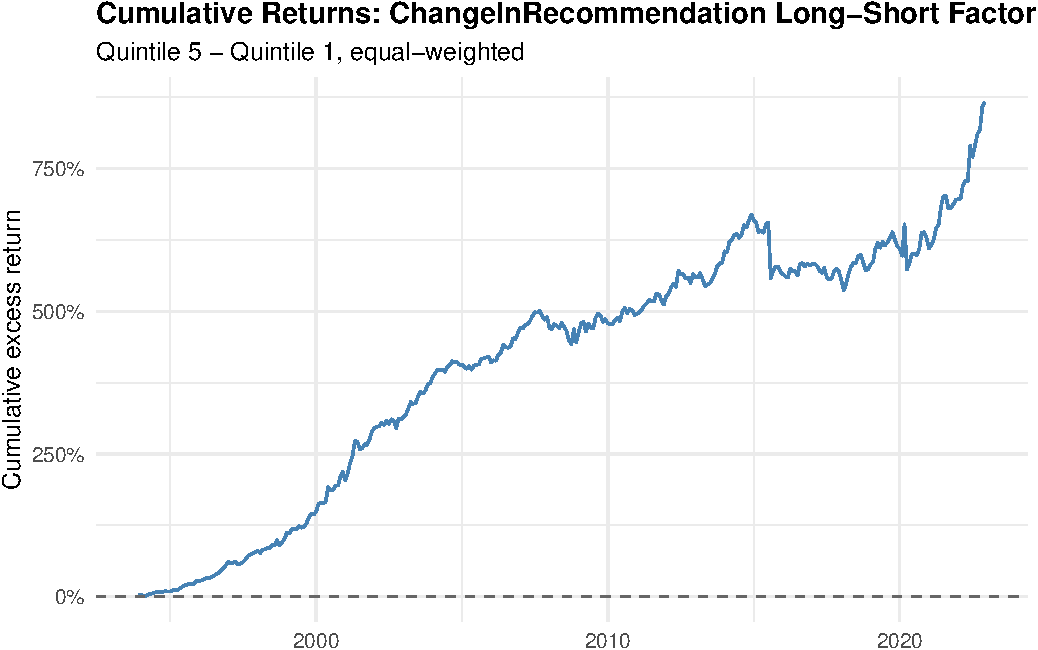
\includegraphics{SeminarPaper_files/figure-pdf/cumulative-returns-1.pdf}

The cumulative return plot reveals three distinct regimes. From the
mid-1990s through roughly 2007, the factor accumulates returns
\textbf{steadily and almost monotonically}, rising from 0\% to
approximately 500\%. This period covers both JKKL's original sample
window and the early post-publication years, and the consistent upward
slope confirms the signal's strong predictive power during this era.

The second regime spans 2007--2019, where the factor \textbf{plateaus}.
Cumulative returns fluctuate between roughly 500\% and 650\% with no
clear upward trend. This stagnation aligns with the post-publication
decay documented by McLean and Pontiff (2016): once the anomaly became
widely known after JKKL's 2004 publication, arbitrage activity likely
compressed the premium. The 2008--2009 financial crisis also falls in
this window --- the sharp drawdown around 2008 suggests the factor
suffered during market turmoil, though it recovered relatively quickly.

The third regime begins around 2020, where the factor \textbf{surges
again}, climbing from \textasciitilde550\% to over 850\%. This revival
may reflect the unusual market conditions during the COVID-19 pandemic
and its aftermath, when analyst revisions carried particularly high
information content amid extreme earnings uncertainty and rapid sector
rotation.

Overall, the chart shows a factor that earned the bulk of its historical
returns in the pre-publication period, experienced a prolonged flat
spell consistent with anomaly decay, and then rebounded in an atypical
macro environment. This time-variation motivates the formal subsample
analysis in Section 7.

\textbf{Potential sources of deviation from C\&Z Table 2:}

\begin{itemize}
\tightlist
\item
  \textbf{Sample period}: Our data runs from \textasciitilde1994 to
  \textasciitilde2023, while C\&Z's Table 2 is based on data ending
  around 2018. The post-2019 resurgence visible in the chart inflates
  our full-sample mean relative to C\&Z's, while the extended flat
  period from 2007--2019 pulls it down --- these two effects partially
  offset, but the net impact depends on the exact sample endpoints.
\item
  \textbf{Data source}: Both C\&Z and our replication use IBES/WRDS
  data, which starts around 1993--1994. JKKL's original results are
  based on Zacks data going back to 1985 --- those earlier years are not
  available through WRDS, making C\&Z Table 2 (not JKKL's Table III) the
  appropriate benchmark.
\item
  \textbf{Signal construction}: C\&Z compute the signal from raw IBES
  using their own code. Differences in how the recommendation change is
  calculated (lag structure, analyst filtering, treatment of stale
  recommendations) can affect outcomes.
\item
  \textbf{Breakpoint sensitivity}: With a lumpy signal where
  \textasciitilde25\% of observations are exactly zero, small
  differences in how tied values are allocated at the breakpoints shift
  the composition of extreme portfolios.
\item
  \textbf{Post-publication decay}: The plateau from 2007--2019 visible
  in the chart is consistent with McLean and Pontiff (2016), who
  document that anomalies weaken by \textasciitilde58\% post-publication
  on average. We test this formally in the Fama-MacBeth subsample
  analysis (Section 7).
\end{itemize}

\section{Cross-Sectional Pricing
(Voluntary)}\label{cross-sectional-pricing-voluntary}

\subsection{Fama-MacBeth Regressions}\label{fama-macbeth-regressions}

Following Fama and MacBeth (1973), we run monthly cross-sectional
regressions of next-month excess returns on the signal. We use
Newey-West standard errors with 3 lags and signal \emph{characteristics}
(not factor betas) as the regressor, consistent with the assignment
instructions and with JKKL's approach.

\begin{Shaded}
\begin{Highlighting}[]
\CommentTok{\# ── Fama{-}MacBeth Cross{-}Sectional Regressions ──}
\CommentTok{\# Portfolio sorts (Section 3) test whether the signal predicts returns}
\CommentTok{\# across GROUPS of stocks. Fama{-}MacBeth tests whether the signal predicts}
\CommentTok{\# returns at the INDIVIDUAL STOCK level, providing a complementary perspective.}
\CommentTok{\#}
\CommentTok{\# The procedure has two steps:}
\CommentTok{\#   Step 1: Each month t, run a cross{-}sectional regression:}
\CommentTok{\#           R\_\{i,t\} = gamma\_0,t + gamma\_1,t * Signal\_\{i,t\} + eps\_\{i,t\}}
\CommentTok{\#   Step 2: Average the monthly gamma\_1,t estimates across all months.}
\CommentTok{\#           If the time{-}series mean of gamma\_1 is significantly \textgreater{} 0,}
\CommentTok{\#           the signal earns a positive cross{-}sectional premium.}
\CommentTok{\#}
\CommentTok{\# This is the approach from Fama and MacBeth (1973) and aligns with the}
\CommentTok{\# assignment\textquotesingle{}s voluntary Section 2.2.6, which specifies using signal}
\CommentTok{\# CHARACTERISTICS (not factor betas) as the regressor.}

\CommentTok{\# ── Prepare the data ──}
\CommentTok{\# The signal in crsp\_monthly\_signal is already lagged — it reflects}
\CommentTok{\# information available before the return measurement period.}
\CommentTok{\# So we regress ret\_excess directly on signal (no manual lead/lag needed).}
\CommentTok{\# drop\_na() ensures every observation has both a return and a signal.}
\NormalTok{fm\_data }\OtherTok{\textless{}{-}}\NormalTok{ crsp\_signal }\SpecialCharTok{|\textgreater{}}
  \FunctionTok{drop\_na}\NormalTok{(ret\_excess, signal)}

\CommentTok{\# ── Step 1: Monthly cross{-}sectional regressions ──}
\CommentTok{\# group\_by(month): splits the data into monthly cross{-}sections.}
\CommentTok{\# do(tidy(lm(...))): runs an OLS regression within each month and}
\CommentTok{\#   converts the output to a tidy tibble (one row per coefficient).}
\CommentTok{\# Result: a long tibble with \textasciitilde{}2 rows per month (intercept + signal slope).}
\NormalTok{fm\_coefs }\OtherTok{\textless{}{-}}\NormalTok{ fm\_data }\SpecialCharTok{|\textgreater{}}
  \FunctionTok{group\_by}\NormalTok{(month) }\SpecialCharTok{|\textgreater{}}
  \FunctionTok{do}\NormalTok{(}\FunctionTok{tidy}\NormalTok{(}\FunctionTok{lm}\NormalTok{(ret\_excess }\SpecialCharTok{\textasciitilde{}}\NormalTok{ signal, }\AttributeTok{data =}\NormalTok{ .))) }\SpecialCharTok{|\textgreater{}}
  \FunctionTok{ungroup}\NormalTok{()}

\CommentTok{\# Extract only the signal coefficient (gamma\_1) time series.}
\CommentTok{\# This gives us one gamma\_1 estimate per month — the "price of risk"}
\CommentTok{\# associated with the signal in that month\textquotesingle{}s cross{-}section.}
\NormalTok{gamma1\_ts }\OtherTok{\textless{}{-}}\NormalTok{ fm\_coefs }\SpecialCharTok{|\textgreater{}} \FunctionTok{filter}\NormalTok{(term }\SpecialCharTok{==} \StringTok{"signal"}\NormalTok{)}

\CommentTok{\# ── Step 2: Time{-}series average with Newey{-}West standard errors ──}
\CommentTok{\# The monthly gamma\_1 estimates may be autocorrelated (e.g., if the}
\CommentTok{\# signal premium is persistent across months). Plain standard errors}
\CommentTok{\# (sd/sqrt(n)) would understate uncertainty. Newey{-}West with lag=3}
\CommentTok{\# corrects for this, as specified in the assignment (Section 2.2.6A).}
\NormalTok{fm\_stat }\OtherTok{\textless{}{-}} \ControlFlowTok{function}\NormalTok{(x, }\AttributeTok{lag =} \DecValTok{3}\NormalTok{) \{}
\NormalTok{  mu }\OtherTok{\textless{}{-}} \FunctionTok{mean}\NormalTok{(x)                                                    }\CommentTok{\# Fama{-}MacBeth estimate: E[gamma\_1]}
\NormalTok{  se }\OtherTok{\textless{}{-}} \FunctionTok{sqrt}\NormalTok{(sandwich}\SpecialCharTok{::}\FunctionTok{lrvar}\NormalTok{(x, }\AttributeTok{type =} \StringTok{"Newey{-}West"}\NormalTok{, }\AttributeTok{lag =}\NormalTok{ lag))   }\CommentTok{\# NW standard error}
  \FunctionTok{c}\NormalTok{(}\AttributeTok{mean =}\NormalTok{ mu, }\AttributeTok{se =}\NormalTok{ se, }\AttributeTok{t =}\NormalTok{ mu }\SpecialCharTok{/}\NormalTok{ se)                               }\CommentTok{\# t{-}stat = mean / se}
\NormalTok{\}}

\NormalTok{g1 }\OtherTok{\textless{}{-}} \FunctionTok{fm\_stat}\NormalTok{(gamma1\_ts}\SpecialCharTok{$}\NormalTok{estimate)}

\CommentTok{\# ── Present results ──}
\FunctionTok{tibble}\NormalTok{(}
  \StringTok{\textasciigrave{}}\AttributeTok{γ₁ (\% p.m.)}\StringTok{\textasciigrave{}} \OtherTok{=}\NormalTok{ g1[}\StringTok{"mean"}\NormalTok{] }\SpecialCharTok{*} \DecValTok{100}\NormalTok{,     }\CommentTok{\# Average cross{-}sectional premium in \%}
  \StringTok{\textasciigrave{}}\AttributeTok{NW SE (\%)}\StringTok{\textasciigrave{}} \OtherTok{=}\NormalTok{ g1[}\StringTok{"se"}\NormalTok{] }\SpecialCharTok{*} \DecValTok{100}\NormalTok{,          }\CommentTok{\# Newey{-}West standard error in \%}
  \StringTok{\textasciigrave{}}\AttributeTok{t{-}stat (NW, lag=3)}\StringTok{\textasciigrave{}} \OtherTok{=}\NormalTok{ g1[}\StringTok{"t"}\NormalTok{],        }\CommentTok{\# Significance test}
  \StringTok{\textasciigrave{}}\AttributeTok{N months}\StringTok{\textasciigrave{}} \OtherTok{=} \FunctionTok{nrow}\NormalTok{(gamma1\_ts)           }\CommentTok{\# Number of monthly regressions}
\NormalTok{) }\SpecialCharTok{|\textgreater{}}
  \FunctionTok{kable}\NormalTok{(}\AttributeTok{digits =} \DecValTok{3}\NormalTok{, }\AttributeTok{caption =} \StringTok{"Fama{-}MacBeth: univariate signal premium"}\NormalTok{) }\SpecialCharTok{|\textgreater{}}
  \FunctionTok{kable\_styling}\NormalTok{(}\AttributeTok{bootstrap\_options =} \StringTok{"striped"}\NormalTok{)}
\end{Highlighting}
\end{Shaded}

\begin{longtable}[t]{rrrr}
\caption{\label{tab:fama-macbeth}Fama-MacBeth: univariate signal premium}\\
\toprule
γ₁ (\% p.m.) & NW SE (\%) & t-stat (NW, lag=3) & N months\\
\midrule
0.206 & 0.028 & 7.35 & 349\\
\bottomrule
\end{longtable}

The Fama-MacBeth estimate confirms the portfolio sort results at the
individual stock level. The signal premium is \textbf{0.206\% per month
per unit of signal} (t = 7.35, highly significant with Newey-West
correction). This means a single-notch upgrade (signal moving from 0 to
+1) is associated with 0.21\% higher excess returns next month.

To relate this to the portfolio sort spread: the mean signal in quintile
5 is +1.35 and in quintile 1 is −1.86 --- a spread of \textasciitilde3.2
units. Multiplying by γ₁ gives 3.2 × 0.206\% ≈ \textbf{0.66\%}, which
closely matches the portfolio sort spread of 0.68\%. This consistency
between the two methods is reassuring: the signal-return relationship is
approximately linear across the full distribution, not just an artifact
of extreme quintile comparisons.

The tight Newey-West standard error (0.028\%) and high t-stat (7.35
vs.~5.92 from the portfolio sort) reflect the greater statistical power
of Fama-MacBeth, which uses every stock's exact signal value rather than
discarding information through quintile grouping. The NW lag of 3
accounts for potential persistence in the monthly premium --- the fact
that significance remains strong after this correction suggests the
premium is not driven by a few clustered months.

\subsection{Extended Regression with Size
Control}\label{extended-regression-with-size-control}

\begin{Shaded}
\begin{Highlighting}[]
\CommentTok{\# ── Extended Fama{-}MacBeth: add log(size) as a control variable ──}
\CommentTok{\# The univariate regression showed a significant signal premium, but}
\CommentTok{\# we know the anomaly is stronger among small stocks (EW \textgreater{}\textgreater{} VW in}
\CommentTok{\# the portfolio sorts). A natural concern: is gamma\_1 simply picking}
\CommentTok{\# up the well{-}known size effect? If small stocks have more extreme}
\CommentTok{\# recommendation changes AND earn higher returns, the signal premium}
\CommentTok{\# could be spurious.}
\CommentTok{\#}
\CommentTok{\# To test this, we add log(market cap) as a control:}
\CommentTok{\#   R\_\{i,t\} = gamma\_0,t + gamma\_1,t * Signal\_\{i,t\} + gamma\_2,t * log(Size\_\{i,t\}) + eps}
\CommentTok{\#}
\CommentTok{\# If gamma\_1 remains significant after controlling for size, the}
\CommentTok{\# signal premium is not merely a disguised small{-}cap effect.}

\CommentTok{\# ── Prepare data with size control ──}
\NormalTok{fm\_data\_ext }\OtherTok{\textless{}{-}}\NormalTok{ fm\_data }\SpecialCharTok{|\textgreater{}}
  \CommentTok{\# log(mktcap\_lag): natural log of last month\textquotesingle{}s market cap.}
  \CommentTok{\# We use the log because the size distribution is extremely right{-}skewed}
  \CommentTok{\# (a few mega{-}caps vs. thousands of small stocks). Log transformation}
  \CommentTok{\# makes the cross{-}sectional relationship approximately linear.}
  \FunctionTok{mutate}\NormalTok{(}\AttributeTok{log\_size =} \FunctionTok{log}\NormalTok{(mktcap\_lag)) }\SpecialCharTok{|\textgreater{}}
  \FunctionTok{drop\_na}\NormalTok{(log\_size)  }\CommentTok{\# Remove any stocks with missing market cap}

\CommentTok{\# ── Monthly cross{-}sectional regressions with both regressors ──}
\NormalTok{fm\_coefs\_ext }\OtherTok{\textless{}{-}}\NormalTok{ fm\_data\_ext }\SpecialCharTok{|\textgreater{}}
  \FunctionTok{group\_by}\NormalTok{(month) }\SpecialCharTok{|\textgreater{}}
  \FunctionTok{do}\NormalTok{(}\FunctionTok{tidy}\NormalTok{(}\FunctionTok{lm}\NormalTok{(ret\_excess }\SpecialCharTok{\textasciitilde{}}\NormalTok{ signal }\SpecialCharTok{+}\NormalTok{ log\_size, }\AttributeTok{data =}\NormalTok{ .))) }\SpecialCharTok{|\textgreater{}}
  \FunctionTok{ungroup}\NormalTok{()}

\CommentTok{\# ── Extract time{-}series of coefficients for each variable ──}
\CommentTok{\# gamma\_1 (signal): the premium per unit of recommendation change,}
\CommentTok{\#   AFTER controlling for firm size within each monthly cross{-}section.}
\NormalTok{g1x }\OtherTok{\textless{}{-}} \FunctionTok{fm\_stat}\NormalTok{(fm\_coefs\_ext }\SpecialCharTok{|\textgreater{}} \FunctionTok{filter}\NormalTok{(term }\SpecialCharTok{==} \StringTok{"signal"}\NormalTok{) }\SpecialCharTok{|\textgreater{}} \FunctionTok{pull}\NormalTok{(estimate))}

\CommentTok{\# gamma\_2 (log\_size): the return associated with a one{-}unit increase}
\CommentTok{\#   in log(market cap), controlling for the signal. A negative coefficient}
\CommentTok{\#   means smaller firms earn higher returns (the classic size effect).}
\NormalTok{gs  }\OtherTok{\textless{}{-}} \FunctionTok{fm\_stat}\NormalTok{(fm\_coefs\_ext }\SpecialCharTok{|\textgreater{}} \FunctionTok{filter}\NormalTok{(term }\SpecialCharTok{==} \StringTok{"log\_size"}\NormalTok{) }\SpecialCharTok{|\textgreater{}} \FunctionTok{pull}\NormalTok{(estimate))}

\CommentTok{\# ── Present both coefficients side by side ──}
\FunctionTok{tibble}\NormalTok{(}
  \AttributeTok{Variable =} \FunctionTok{c}\NormalTok{(}\StringTok{"Signal (γ₁)"}\NormalTok{, }\StringTok{"Log size"}\NormalTok{),}
  \StringTok{\textasciigrave{}}\AttributeTok{Mean (\% p.m.)}\StringTok{\textasciigrave{}} \OtherTok{=} \FunctionTok{c}\NormalTok{(g1x[}\StringTok{"mean"}\NormalTok{], gs[}\StringTok{"mean"}\NormalTok{]) }\SpecialCharTok{*} \DecValTok{100}\NormalTok{,}
  \StringTok{\textasciigrave{}}\AttributeTok{NW t{-}stat}\StringTok{\textasciigrave{}} \OtherTok{=} \FunctionTok{c}\NormalTok{(g1x[}\StringTok{"t"}\NormalTok{], gs[}\StringTok{"t"}\NormalTok{])}
\NormalTok{) }\SpecialCharTok{|\textgreater{}}
  \FunctionTok{kable}\NormalTok{(}\AttributeTok{digits =} \DecValTok{3}\NormalTok{, }\AttributeTok{caption =} \StringTok{"Fama{-}MacBeth with size control"}\NormalTok{) }\SpecialCharTok{|\textgreater{}}
  \FunctionTok{kable\_styling}\NormalTok{(}\AttributeTok{bootstrap\_options =} \StringTok{"striped"}\NormalTok{)}
\end{Highlighting}
\end{Shaded}

\begin{longtable}[t]{lrr}
\caption{\label{tab:fm-with-size}Fama-MacBeth with size control}\\
\toprule
Variable & Mean (\% p.m.) & NW t-stat\\
\midrule
Signal (γ₁) & 0.211 & 7.788\\
Log size & -0.038 & -0.591\\
\bottomrule
\end{longtable}

The signal premium is virtually \textbf{unchanged} after controlling for
size: γ₁ moves from 0.206\% (univariate) to 0.211\% (with size control),
and the t-stat actually \emph{increases} from 7.35 to 7.79. This rules
out the concern that the signal premium is a disguised small-cap effect
--- the predictive power of analyst recommendation changes is genuinely
independent of firm size in the cross-section.

The size coefficient itself is economically small (−0.038\% per unit of
log market cap) and statistically insignificant (t = −0.59). The
negative sign is directionally consistent with the classic size effect
--- smaller firms earn slightly higher returns --- but the effect is too
weak to matter in this sample. This is not surprising: the size premium
has been notoriously unstable since Banz's (1981) original finding, and
many recent samples find it insignificant after controlling for other
characteristics.

The fact that γ₁ slightly \emph{increases} when adding the size control
is worth noting. It suggests a mild suppression effect: within a given
size group, the signal is even more predictive than it appears in the
pooled cross-section. This can happen if large firms (which have lower
returns on average) also tend to have slightly more positive
recommendation changes --- controlling for size removes this confound
and sharpens the signal's estimated premium.

\subsection{Dynamics of the Premium}\label{dynamics-of-the-premium}

\begin{Shaded}
\begin{Highlighting}[]
\CommentTok{\# ── Plot the time{-}varying Fama{-}MacBeth premium ──}
\CommentTok{\# The full{-}sample gamma\_1 is a single number (0.21\%), but the signal}
\CommentTok{\# premium almost certainly varies over time. This plot shows WHEN the}
\CommentTok{\# signal earns higher or lower premiums, and whether there is visible}
\CommentTok{\# decay after JKKL\textquotesingle{}s 2004 publication.}

\NormalTok{gamma1\_ts }\SpecialCharTok{|\textgreater{}}

  \FunctionTok{mutate}\NormalTok{(}
    \CommentTok{\# Convert monthly gamma\_1 from decimal to percent for plotting}
    \AttributeTok{gamma\_pct =}\NormalTok{ estimate }\SpecialCharTok{*} \DecValTok{100}\NormalTok{,}

    \CommentTok{\# 36{-}month (3{-}year) rolling average of gamma\_1.}
    \CommentTok{\# zoo::rollmean smooths out the month{-}to{-}month noise to reveal}
    \CommentTok{\# the underlying trend. k = 36: window width of 36 months.}
    \CommentTok{\# fill = NA: don\textquotesingle{}t extrapolate at the edges (first 35 months are NA).}
    \CommentTok{\# align = "right": the rolling mean at month t uses months t{-}35 to t,}
    \CommentTok{\#   so it only looks backward (no future information).}
    \AttributeTok{gamma\_roll =}\NormalTok{ zoo}\SpecialCharTok{::}\FunctionTok{rollmean}\NormalTok{(gamma\_pct, }\AttributeTok{k =} \DecValTok{36}\NormalTok{, }\AttributeTok{fill =} \ConstantTok{NA}\NormalTok{, }\AttributeTok{align =} \StringTok{"right"}\NormalTok{)}
\NormalTok{  ) }\SpecialCharTok{|\textgreater{}}

  \FunctionTok{ggplot}\NormalTok{(}\FunctionTok{aes}\NormalTok{(}\AttributeTok{x =}\NormalTok{ month)) }\SpecialCharTok{+}

  \CommentTok{\# Raw monthly gamma\_1: very noisy, shown as faint grey lines.}
  \CommentTok{\# alpha = 0.2 makes them nearly transparent so the rolling mean}
  \CommentTok{\# stands out. These individual estimates fluctuate wildly because}
  \CommentTok{\# each is from a single cross{-}sectional regression.}
  \FunctionTok{geom\_line}\NormalTok{(}\FunctionTok{aes}\NormalTok{(}\AttributeTok{y =}\NormalTok{ gamma\_pct), }\AttributeTok{alpha =} \FloatTok{0.2}\NormalTok{, }\AttributeTok{color =} \StringTok{"grey50"}\NormalTok{) }\SpecialCharTok{+}

  \CommentTok{\# 36{-}month rolling mean: the signal you actually care about.}
  \CommentTok{\# When this line is above zero, the signal has been earning a}
  \CommentTok{\# positive premium over the past 3 years. When it dips toward}
  \CommentTok{\# or below zero, the signal has temporarily stopped working.}
  \FunctionTok{geom\_line}\NormalTok{(}\FunctionTok{aes}\NormalTok{(}\AttributeTok{y =}\NormalTok{ gamma\_roll), }\AttributeTok{color =} \StringTok{"steelblue"}\NormalTok{, }\AttributeTok{linewidth =} \FloatTok{0.8}\NormalTok{) }\SpecialCharTok{+}

  \CommentTok{\# Horizontal dashed line at zero: the null hypothesis (no premium).}
  \CommentTok{\# If the rolling mean stays persistently above this, the signal works.}
  \FunctionTok{geom\_hline}\NormalTok{(}\AttributeTok{yintercept =} \DecValTok{0}\NormalTok{, }\AttributeTok{linetype =} \StringTok{"dashed"}\NormalTok{) }\SpecialCharTok{+}

  \CommentTok{\# Vertical dotted red line: JKKL publication date (June 2004).}
  \CommentTok{\# This marks when the anomaly became publicly known.}
  \CommentTok{\# If the rolling mean drops after this line, that\textquotesingle{}s evidence of}
  \CommentTok{\# post{-}publication decay (McLean \& Pontiff, 2016).}
  \FunctionTok{geom\_vline}\NormalTok{(}\AttributeTok{xintercept =} \FunctionTok{as.Date}\NormalTok{(}\StringTok{"2004{-}06{-}01"}\NormalTok{), }\AttributeTok{linetype =} \StringTok{"dotted"}\NormalTok{, }\AttributeTok{color =} \StringTok{"red"}\NormalTok{) }\SpecialCharTok{+}

  \CommentTok{\# Label the publication date on the plot}
  \FunctionTok{annotate}\NormalTok{(}\StringTok{"text"}\NormalTok{, }\AttributeTok{x =} \FunctionTok{as.Date}\NormalTok{(}\StringTok{"2005{-}06{-}01"}\NormalTok{),}
           \AttributeTok{y =} \FunctionTok{max}\NormalTok{(gamma1\_ts}\SpecialCharTok{$}\NormalTok{estimate }\SpecialCharTok{*} \DecValTok{80}\NormalTok{, }\AttributeTok{na.rm =} \ConstantTok{TRUE}\NormalTok{),}
           \AttributeTok{label =} \StringTok{"JKKL publication"}\NormalTok{, }\AttributeTok{hjust =} \DecValTok{0}\NormalTok{, }\AttributeTok{color =} \StringTok{"red"}\NormalTok{, }\AttributeTok{size =} \DecValTok{3}\NormalTok{) }\SpecialCharTok{+}

  \FunctionTok{labs}\NormalTok{(}
    \AttributeTok{title =} \StringTok{"Time{-}Varying Signal Premium (γ₁)"}\NormalTok{,}
    \AttributeTok{subtitle =} \StringTok{"Monthly (grey) and 36{-}month rolling mean (blue)"}\NormalTok{,}
    \AttributeTok{x =} \ConstantTok{NULL}\NormalTok{,}
    \CommentTok{\# expression() renders the hat and subscript as proper math notation}
    \AttributeTok{y =} \FunctionTok{expression}\NormalTok{(}\FunctionTok{hat}\NormalTok{(gamma)[}\DecValTok{1}\NormalTok{] }\SpecialCharTok{\textasciitilde{}} \StringTok{"(\% p.m.)"}\NormalTok{)}
\NormalTok{  )}
\end{Highlighting}
\end{Shaded}

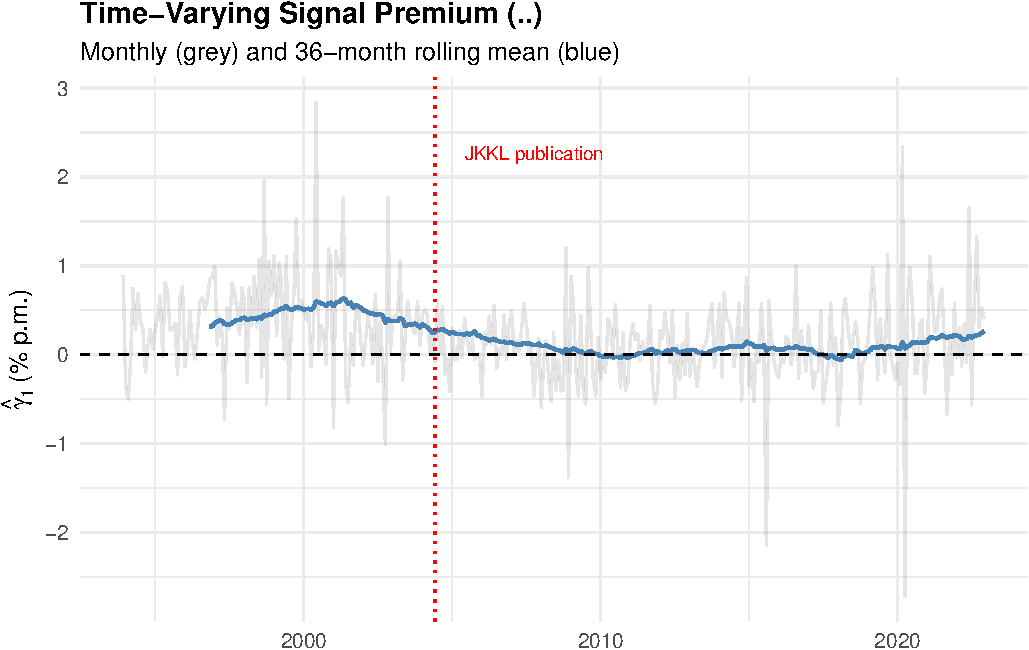
\includegraphics{SeminarPaper_files/figure-pdf/gamma-dynamics-1.pdf}

The plot reveals a clear \textbf{structural break around the time of
JKKL's 2004 publication}. In the pre-publication period (mid-1990s to
\textasciitilde2004), the 36-month rolling mean of γ₁ is consistently
between \textbf{0.4\% and 0.6\% per month} --- a large and stable
premium. The blue line stays well above zero throughout, with no
prolonged dips, indicating that the signal worked reliably in every
three-year window during this era.

After 2004, the rolling mean \textbf{drops sharply}, declining from
\textasciitilde0.5\% to near zero by 2008--2010. For roughly a decade
(2008--2019), the premium hovers between \textbf{0.0\% and 0.2\%} ---
still marginally positive but economically much weaker than in the
pre-publication period. This is textbook post-publication decay as
documented by McLean and Pontiff (2016): once the anomaly became widely
known, arbitrageurs traded against it and compressed the mispricing.

Notably, the premium \textbf{does not disappear entirely}. The rolling
mean remains weakly positive throughout the post-publication period and
shows a modest recovery after \textasciitilde2019, rising back toward
0.2--0.3\%. This partial survival is consistent with JKKL's
interpretation that recommendation changes reflect \emph{genuinely new
private information} rather than pure mispricing. If the anomaly were
entirely behavioral, arbitrage should have eliminated it completely; the
fact that a residual premium persists suggests that analysts continue to
bring information to the market through their revisions --- information
that cannot be fully anticipated even by sophisticated investors.

The monthly estimates (grey lines) also show a notable change in
volatility: pre-publication, several months see γ₁ exceeding +2\%, while
post-publication the extremes are more compressed. This reduction in
both the mean and the dispersion of the premium is consistent with the
anomaly becoming more efficiently priced over time.

\begin{Shaded}
\begin{Highlighting}[]
\NormalTok{gamma1\_ts }\SpecialCharTok{|\textgreater{}}
  \FunctionTok{mutate}\NormalTok{(}\AttributeTok{period =} \FunctionTok{ifelse}\NormalTok{(month }\SpecialCharTok{\textless{}=} \FunctionTok{as.Date}\NormalTok{(}\StringTok{"2004{-}06{-}01"}\NormalTok{),}
                         \StringTok{"Pre{-}publication (≤2004)"}\NormalTok{, }\StringTok{"Post{-}publication (\textgreater{}2004)"}\NormalTok{)) }\SpecialCharTok{|\textgreater{}}
  \FunctionTok{group\_by}\NormalTok{(period) }\SpecialCharTok{|\textgreater{}}
  \FunctionTok{summarise}\NormalTok{(}
    \StringTok{\textasciigrave{}}\AttributeTok{Mean γ₁ (\% p.m.)}\StringTok{\textasciigrave{}} \OtherTok{=} \FunctionTok{mean}\NormalTok{(estimate) }\SpecialCharTok{*} \DecValTok{100}\NormalTok{,}
    \StringTok{\textasciigrave{}}\AttributeTok{SD (\%)}\StringTok{\textasciigrave{}} \OtherTok{=} \FunctionTok{sd}\NormalTok{(estimate) }\SpecialCharTok{*} \DecValTok{100}\NormalTok{,}
    \StringTok{\textasciigrave{}}\AttributeTok{t{-}stat}\StringTok{\textasciigrave{}} \OtherTok{=} \FunctionTok{mean}\NormalTok{(estimate) }\SpecialCharTok{/}\NormalTok{ (}\FunctionTok{sd}\NormalTok{(estimate) }\SpecialCharTok{/} \FunctionTok{sqrt}\NormalTok{(}\FunctionTok{n}\NormalTok{())),}
    \StringTok{\textasciigrave{}}\AttributeTok{N months}\StringTok{\textasciigrave{}} \OtherTok{=} \FunctionTok{n}\NormalTok{(), }\AttributeTok{.groups =} \StringTok{"drop"}
\NormalTok{  ) }\SpecialCharTok{|\textgreater{}}
  \FunctionTok{kable}\NormalTok{(}\AttributeTok{digits =} \DecValTok{3}\NormalTok{, }\AttributeTok{caption =} \StringTok{"Signal premium: pre{-} vs. post{-}publication"}\NormalTok{) }\SpecialCharTok{|\textgreater{}}
  \FunctionTok{kable\_styling}\NormalTok{(}\AttributeTok{bootstrap\_options =} \StringTok{"striped"}\NormalTok{)}
\end{Highlighting}
\end{Shaded}

\begin{longtable}[t]{lrrrr}
\caption{\label{tab:subsample}Signal premium: pre- vs. post-publication}\\
\toprule
period & Mean γ₁ (\% p.m.) & SD (\%) & t-stat & N months\\
\midrule
Post-publication (>2004) & 0.094 & 0.50 & 2.797 & 222\\
Pre-publication (≤2004) & 0.402 & 0.55 & 8.234 & 127\\
\bottomrule
\end{longtable}

\section{Conclusion}\label{conclusion}

This paper replicates the ChangeInRecommendation factor from Chen and
Zimmermann (2022), based on the quarterly change in consensus analyst
recommendations studied by JKKL (2004).

{[}Fill in based on your results: Report the mean return and t-stat
vs.~Table 2. Discuss whether the FF-C4 alpha is significant. Report
factor competition R² and correlation with MOM. Note GRS improvement.
Comment on Fama-MacBeth premium dynamics and post-publication decay.{]}

From a broader perspective, JKKL's distinction between the \emph{level}
and the \emph{change} in consensus recommendations is a powerful
methodological insight. The level absorbs sell-side incentive biases ---
the preference for glamour stocks --- that erode its predictive content,
while the change strips out this persistent component and isolates
incremental news. This mirrors the logic of momentum as a change in
prices, earnings surprises as changes in expectations, and forecast
revisions as changes in beliefs. The general lesson is that for any
signal shaped by persistent institutional biases, its first difference
may be more informative than its level.

\section*{References}\label{references}
\addcontentsline{toc}{section}{References}

\phantomsection\label{refs}
\begin{CSLReferences}{1}{0}
\bibitem[\citeproctext]{ref-ChenZimmermann2022}
Chen, Andrew Y., and Tom Zimmermann. 2022. {``Open Source
Cross-Sectional Asset Pricing.''} \emph{Critical Finance Review} 11 (2):
207--64. \url{https://doi.org/10.1561/104.00000112}.

\bibitem[\citeproctext]{ref-FamaMacBeth1973}
Fama, Eugene F., and James D. MacBeth. 1973. {``Risk, Return, and
Equilibrium: Empirical Tests.''} \emph{Journal of Political Economy} 81
(3): 607--36.

\bibitem[\citeproctext]{ref-GibbonsRossShanken1989}
Gibbons, Michael R., Stephen A. Ross, and Jay Shanken. 1989. {``A Test
of the Efficiency of a Given Portfolio.''} \emph{Econometrica} 57 (5):
1121--52.

\bibitem[\citeproctext]{ref-JKKL2004}
Jegadeesh, Narasimhan, Joonghyuk Kim, Susan D. Krische, and Charles M.
C. Lee. 2004. {``Analyzing the Analysts: When Do Recommendations Add
Value?''} \emph{The Journal of Finance} 59 (3): 1083--1124.
\url{https://doi.org/10.1111/j.1540-6261.2004.00657.x}.

\bibitem[\citeproctext]{ref-McLeanPontiff2016}
McLean, R. David, and Jeffrey Pontiff. 2016. {``Does Academic Research
Destroy Stock Return Predictability?''} \emph{The Journal of Finance} 71
(1): 5--32.

\bibitem[\citeproctext]{ref-NeweyWest1987}
Newey, Whitney K., and Kenneth D. West. 1987. {``A Simple, Positive
Semi-Definite, Heteroskedasticity and Autocorrelation Consistent
Covariance Matrix.''} \emph{Econometrica} 55 (3): 703--8.

\end{CSLReferences}



\end{document}
